\documentclass[12pt,twoside,a4paper]{book}

% Language setting
% Replace `english' with e.g. `spanish' to change the document language
\usepackage[galician]{babel}

% Set page size and margins
% Replace `letterpaper' with `a4paper' for UK/EU standard size
\usepackage[letterpaper,top=2cm,bottom=2cm,left=3cm,right=3cm,marginparwidth=1.75cm]{geometry}

\date{Febreiro 2026}

\usepackage[colorlinks=true, allcolors=blue]{hyperref}
\usepackage[T1]{fontenc}

\usepackage{titlesec}
\usepackage{booktabs}
\usepackage{tabularx}
\usepackage{longtable}
\usepackage{graphicx}
\usepackage{xcolor}
\usepackage{float}
\usepackage{caption}
\usepackage{subcaption}
\usepackage{enumitem}
\usepackage{pifont}
\usepackage{listings}

\graphicspath{{.}{diagrams/}{screenshots/}}
\definecolor{uscred}{RGB}{128,0,0}

% Índice ata subsubsección (os casos de uso, en \paragraph, non aparecen no índice)
\setcounter{tocdepth}{3}

% Nome do capítulo de bibliografía (clase book)
\renewcommand{\bibname}{Bibliografía}

% Marcador de captura de pantalla pendente (manual de usuario).
% Para inserir a imaxe real, substituír a liña \fbox{...} por:
%   \includegraphics[width=0.45\textwidth]{screenshots/<ficheiro>}
\newcommand{\figcaptura}[2]{%
  \begin{figure}[H]\centering
  \fbox{\parbox[c][4.5cm][c]{0.5\textwidth}{\centering\itshape [Captura de pantalla pendente]\\[4pt]#1}}%
  \caption{#1}\label{#2}\end{figure}}

% --- Paleta de cores de Telaria (figura de deseño visual, §4.6) ---
\definecolor{telPrimary}{HTML}{8b3ce0}
\definecolor{telSecondary}{HTML}{f59e0b}
\definecolor{telWarning}{HTML}{dc2626}
\definecolor{telLbg}{HTML}{f7f3ff}
\definecolor{telLui}{HTML}{ede3fd}
\definecolor{telLtext}{HTML}{3d1e7a}
\definecolor{telLtint}{HTML}{7c3aed}
\definecolor{telLborder}{HTML}{d4c2f9}
\definecolor{telDbg}{HTML}{07050f}
\definecolor{telDui}{HTML}{0e0b1f}
\definecolor{telDtext}{HTML}{e8e0fa}
\definecolor{telDtint}{HTML}{a855f7}
\definecolor{telDborder}{HTML}{2b1650}
\definecolor{swframe}{gray}{0.65}
% Mostra de cor: caixa coloreada + etiqueta hexadecimal
\newcommand{\swatch}[2]{%
  \begin{tabular}{@{}c@{}}
    \fcolorbox{swframe}{#1}{\rule{22pt}{0pt}\rule{0pt}{16pt}}\\[1pt]
    {\scriptsize\texttt{#2}}%
  \end{tabular}%
}

% Estilo base para fragmentos de código (manuais técnicos)
\definecolor{codebg}{RGB}{245,245,245}
\lstset{
  basicstyle=\ttfamily\footnotesize,
  backgroundcolor=\color{codebg},
  breaklines=true,
  frame=single,
  framesep=4pt,
  columns=fullflexible,
  showstringspaces=false,
  captionpos=b,
  extendedchars=true,
  literate=%
    {á}{{\'a}}1 {é}{{\'e}}1 {í}{{\'i}}1 {ó}{{\'o}}1 {ú}{{\'u}}1
    {Á}{{\'A}}1 {É}{{\'E}}1 {Í}{{\'I}}1 {Ó}{{\'O}}1 {Ú}{{\'U}}1
    {ñ}{{\~n}}1 {Ñ}{{\~N}}1 {ü}{{\"u}}1 {ç}{{\c c}}1 {º}{{\textordmasculine}}1,
}


\title{Telaria}
\author{Jorge Otero Pailos}

\begin{document}

% ====================== Portada (formato oficial ETSE) ========================
\pagestyle{empty}
\begin{center}
	{\bf\Large UNIVERSIDADE DE SANTIAGO DE COMPOSTELA}

	\vspace{0.5cm}
	
\includegraphics[width=5cm]{assets/usc/logo_usc.pdf}

	\vspace{0.5cm}
	{\bf\large ESCOLA TÉCNICA SUPERIOR DE ENXEÑARÍA}

	\vspace{3cm}
	{\bf\LARGE Telaria}

	\vspace{0.5cm}
	{\bf\Large Aplicación móbil colaborativa para a xestión integral de viaxes en grupo}
\end{center}

\vspace{2cm}
\hspace{4cm}\begin{tabular}{l}
	{\it\Large Autor:} \\
	{\bf\Large Jorge Otero Pailos} \\
	~ \\
	{\it\Large Titores:} \\
	{\bf\Large Pedro Gamallo Fernández} \\
	{\bf\Large Víctor José Gallego Fontenla}
\end{tabular}

\vspace{2cm}
\begin{center}
	{\bf\Large Grao en Enxeñaría Informática}

	\vspace{0.5cm}
	{\bf\large Xuño 2026}

	\vspace{0.5cm}
	Traballo de Fin de Grao presentado na Escola Técnica Superior de Enxeñaría da Universidade de Santiago de Compostela para a obtención do Grao en Enxeñaría Informática
\end{center}
\cleardoublepage

% ====================== Páxinas previas (numeración romana) ===================
\pagenumbering{roman}
\pagestyle{plain}
\chapter*{Agradecementos}

Quero expresar o meu sinceiro agradecemento a todas as persoas que me apoiaron 
e me axudaron nestre proxecto. En primeiro lugar, á universidade, á facultade e aos 
meus titores por ensinarme todo o necesario pra a realización deste traballo e 
brindarme esta oportunidade. En segundo lugar, á miña familia, parella e amigos
por todo o demáis.
\cleardoublepage
\section{Resumo}

Este Traballo de Fin de Grao ten como obxectivo o deseño e desenvolvemento de
\textbf{Telaria}, unha aplicación móbil colaborativa para a xestión integral de
viaxes en grupo. A aplicación permite coordinar de forma centralizada todos os
aspectos dunha viaxe compartida: o seguimento de gastos e débedas entre os
participantes, a planificación de eventos mediante un calendario común, o
almacenamento de documentos relevantes, a comunicación entre os membros mediante
un chat de grupo e a asistencia dun chatbot conversacional baseado en intelixencia
artificial.

A implementación levouse a cabo empregando tecnoloxías modernas para o
desenvolvemento de aplicacións móbiles multiplataforma, concretamente
\textbf{React Native} con \textbf{Expo} no frontend e \textbf{Spring Boot}
no backend, seguindo unha arquitectura \textit{API-first} baseada na
especificación \textbf{OpenAPI}. A infraestrutura inclúe ademais servizos
de almacenamento de ficheiros, modelos de linguaxe locais e despregamento mediante contedores.

Como conclusión, o proxecto ofrece unha solución completa ao problema de
coordinación habitual nas viaxes en grupo, integrando nunha única plataforma
funcionalidades que adoitan xestionarse de forma dispersa entre distintas
ferramentas.

\cleardoublepage

\tableofcontents
\listoffigures
\listoftables

% ====================== Núcleo da memoria (≤ 50 páxinas) ======================
\cleardoublepage
\pagenumbering{arabic}
\setcounter{page}{1}
\pagestyle{headings}
\chapter{Introdución}

O obxectivo principal deste traballo é o deseño e desenvolvemento de \textbf{Telaria},
unha aplicación móbil colaborativa para a xestión integral de viaxes en grupo. A idea
de partida é sinxela: ofrecer un \textit{espazo de viaxe} único e compartido no que un
grupo de persoas poida organizar todo o ciclo de vida dunha viaxe (antes, durante e despois) sen
ter que interactuar con media ducia de aplicacións xenéricas non pensadas para ese fin.

\section{Motivación e contexto}

A organización dunha viaxe en grupo é, na práctica, un problema de coordinación entre
varias persoas que comparten un mesmo obxectivo pero usan ferramentas distintas e
illadas entre si. Durante a fase de planificación adóitanse acumular as reservas de
aloxamento e transporte no correo ou na galería de cada quen, os horarios nun calendario
persoal e as propostas de actividades nun grupo de mensaxería. Xa durante a viaxe,
súmanse a ese caos os tíckets dos gastos compartidos e as fotos dos documentos
importantes. Ningunha desas ferramentas foi concibida para o contexto concreto dunha
viaxe, polo que a información queda repartida e desactualizada.

Esta fragmentación tradúcese en custos reais para o grupo. O máis evidente é o
económico: ao final da viaxe ninguén sabe con certeza canto puxo cada persoa nin como
saldar as contas, e a liquidación faise a man, de forma propensa a erros e a
transferencias innecesarias. A iso engádese a perda de información (un billete esquecido
no fondo dun fío de chat de centos de mensaxes), a dependencia dunha única persoa que «leva» a
organización e a dificultade de que todos os participantes teñan unha visión completa e
actualizada do plan.

A utilidade que persigue Telaria é precisamente eliminar ese traballo de
coordinación manual. Ao reunir gastos, calendario, documentos, comunicación e asistencia
intelixente nun mesmo espazo compartido por viaxe, cada participante accede sempre á
mesma información actualizada e o esforzo de mantela sincronizada desaparece. O público
ao que se dirixe non é o da viaxe corporativa nin o das axencias, senón os grupos
informais (cuadrillas de amizades, familias ou compañeiros) que viaxan xuntos de cando
en vez e que hoxe resolven esta coordinación cun conxunto disperso de aplicacións
xenéricas.

\section{Solucións existentes e diferenciación}

No mercado existen aplicacións que cobren \textit{partes} do problema descrito, pero
ningunha o aborda de forma integrada para o contexto dunha viaxe en grupo. As
alternativas máis representativas son as seguintes:

\begin{itemize}
  \item \textbf{Tricount}~\cite{tricount}: especializada na xestión de gastos
        compartidos e no cálculo de quen debe a quen. Resolve ben a parte económica, pero
        non ofrece calendario, almacenamento de documentos, chat de grupo nin asistencia
        intelixente. Foi, de feito, unha das inspiracións do proxecto: o seu enfoque da
        liquidación de gastos é o punto de partida que Telaria estende ao resto de
        necesidades dunha viaxe.
  \item \textbf{WhatsApp e grupos de mensaxería}~\cite{whatsapp}: cobren a comunicación
        do grupo, que é onde acaba converxendo o resto da organización por falta dun lugar
        mellor. Todo o demais (gastos, calendario, documentos) queda como información non
        estruturada dentro do fío de conversa, sen ningún tratamento específico.
  \item \textbf{Google Calendar}~\cite{googlecalendar}: resolve a planificación temporal,
        pero é unha ferramenta de calendario xenérica e centrada no individuo, non un
        espazo colaborativo organizado por viaxe nin integrado co resto de necesidades.
  \item \textbf{Wanderlog e TravelPerk}~\cite{wanderlog,travelperk}: son planificadores
        de viaxe máis completos, pero orientados respectivamente ao descubrimento de
        itinerarios e á xestión de viaxes corporativas. Teñen un soporte feble da
        liquidación de gastos compartidos entre iguais e carecen dun asistente de
        intelixencia artificial integrado.
\end{itemize}

A diferenza destas opcións, Telaria integra todas as funcionalidades relevantes nun mesmo produto e engade catro
trazos que a distinguen: \textbf{(1)} un \textit{espazo de viaxe único} que reúne nun
só lugar gastos, calendario, documentos, chat e asistente; \textbf{(2)} un \textit{modelo
plenamente colaborativo sen roles}, no que todos os membros teñen as mesmas capacidades e
ningún depende dun «organizador»; \textbf{(3)} a \textit{liquidación automática con
minimización de débedas}, que reduce ao mínimo o número de transferencias necesarias; e
\textbf{(4)} un \textit{asistente de intelixencia artificial integrado por viaxe}, que
ningunha das alternativas ofrece. O cadro~\ref{tab:comparativa} resume esta comparación.

\begin{table}[H]
  \caption{Comparativa de funcionalidades entre Telaria e as alternativas existentes.}
  \label{tab:comparativa}
  \centering
  \resizebox{\textwidth}{!}{%
  \begin{tabular}{@{}lccccc@{}}
    \toprule
    \textbf{Funcionalidade} & \textbf{Tricount} & \textbf{WhatsApp} & \textbf{G. Calendar} & \textbf{Wanderlog} & \textbf{Telaria} \\
    \midrule
    Gastos e liquidación   & \ding{51} & \ding{55} & \ding{55} & parcial   & \ding{51} \\
    Calendario / eventos   & \ding{55} & \ding{55} & \ding{51} & \ding{51} & \ding{51} \\
    Documentos compartidos & \ding{55} & parcial   & \ding{55} & parcial   & \ding{51} \\
    Chat de grupo          & \ding{55} & \ding{51} & \ding{55} & \ding{55} & \ding{51} \\
    Asistente de IA        & \ding{55} & \ding{55} & \ding{55} & \ding{55} & \ding{51} \\
    Modelo colaborativo    & parcial   & parcial   & \ding{55} & \ding{51} & \ding{51} \\
    \bottomrule
  \end{tabular}}
\end{table}

\section{Obxectivos e descrición do sistema}

Telaria é unha aplicación móbil orientada a grupos de persoas que realizan viaxes
conxuntas. Calquera usuario pode rexistrarse na plataforma e, a partir de aí, crear
novas viaxes ou unirse a viaxes existentes mediante invitación, solicitude ou código QR.

Dentro de cada viaxe, todos os membros teñen acceso completo e en igualdade de
condicións ás funcionalidades da aplicación. Non existe distinción de roles: o sistema
está deseñado baixo un modelo plenamente colaborativo no que calquera participante pode
rexistrar gastos, crear eventos, subir documentos, enviar mensaxes ao chat e interactuar
co asistente de IA. A continuación descríbense, dende o punto de vista do usuario, as
principais funcionalidades que compoñen este espazo de viaxe, cuxa implementación consiste no
principal obxectivo deste traballo.

\begin{figure}[H]
  \centering
  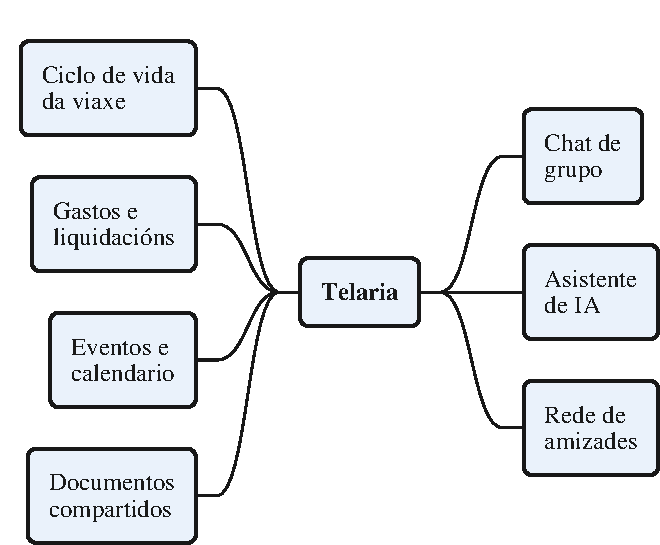
\includegraphics[width=0.80\textwidth]{diagrams/funcionalidades-telaria.pdf}
  \caption{Funcionalidades principais de Telaria.}
  \label{fig:funcionalidades-telaria}
\end{figure}

\textbf{Ciclo de vida da viaxe.} A viaxe é a unidade central arredor da que se organiza
todo o demais. Un usuario crea unha viaxe e convida a outras persoas, que poden
incorporarse por invitación directa, solicitando o acceso ou escaneando un código QR;
calquera membro pode abandonala e xestionar as solicitudes pendentes.

\textbf{Gastos e liquidacións.} Cada membro pode rexistrar os gastos que paga, indicando
os beneficiarios e unha categoría (aloxamento, transporte, comida, etc.). A partir deses
rexistros, o módulo calcula automaticamente o balance de cada persoa e propón un conxunto
de liquidacións aplicando un algoritmo de minimización de débedas, de xeito que o número
de transferencias necesarias para saldar todos os saldos sexa o mínimo posible. As
liquidacións xa realizadas consérvanse nun historial.

\textbf{Eventos e calendario.} O grupo constrúe un itinerario común sobre un calendario
compartido. Cada evento pode ter data, hora, duración e unha localización xeográfica,
que se pode escoller buscando un enderezo ou seleccionándoo directamente nun mapa
interactivo.

\textbf{Documentos compartidos.} A viaxe dispón dun repositorio de documentos relevantes
(reservas, billetes, fotos, etc.) que calquera membro pode subir, descargar ou eliminar.
Para os documentos de imaxe xérase de forma asíncrona unha miniatura de previsualización,
de modo que a listaxe se mostre con axilidade sen descargar os ficheiros orixinais.

\textbf{Chat de grupo.} Cada viaxe inclúe unha sala de conversa propia para a
coordinación entre os membros, con entrega de mensaxes en tempo real e aviso de mensaxes
sen ler. As mensaxes son almacenadas no servidor durante 30 días
e despois son eliminadas automaticamente.

\textbf{Asistente de intelixencia artificial.} Cada viaxe conta cun asistente
conversacional que axuda na planificación e responde consultas. Mantén un historial de
conversa independente por viaxe e por usuario, de modo que o contexto se preserve entre sesións.
Por razóns de rendemento do modelo local, este só recibe como contexto as últimas 5 mensaxes do
chat (ademais do contexto da viaxe),
se ben as demais mensaxes quedan almacenadas e dispoñibles para consulta. O historial completo de conversa mantense durante 30 días.

\textbf{Rede de amizades e xestión de conta.} De maneira complementaria, a plataforma
ofrece unha rede de amizades entre usuarios: calquera usuario pode engadir outros como
amigos e, a partir de aí, convidalos ás súas viaxes de forma máis áxil que mediante o
identificador ou o código QR. Esta funcionalidade non altera o modelo colaborativo
descrito, senón que actúa como atallo para os usuarios habituais. Cada usuario xestiona
ademais o seu propio perfil (nome, correo, avatar e contrasinal) e pode eliminar a súa
conta, operación que require a confirmación do contrasinal. A aplicación está dispoñible
en tres idiomas (galego, español e inglés) e ofrece temas de aparencia clara e escura.

Como obxectivos técnicos, o proxecto busca aplicar unha arquitectura
\textit{API-first} e tecnoloxías multiplataforma modernas, de xeito que a solución
sexa funcional tanto en iOS como en Android dende unha única base de código.

\section{Relación da documentación que conforma a memoria}

\begin{tabularx}{\textwidth}{@{}lX@{}}
  \toprule
  \textbf{Sección} & \textbf{Contido} \\
  \midrule
  Resumo                            & Breve resumo das principais contribucións do traballo. \\[4pt]
  Introdución                       & Obxectivos xerais, descrición do sistema e tecnoloxías e arquitecturas empregadas. \\[4pt]
  Especificación de Requisitos      & Requisitos funcionais e non funcionais, interfaces con outros sistemas e información que o sistema debe almacenar. \\[4pt]
  Deseño                            & Arquitectura do sistema, división en compoñentes e comunicación entre eles. Equipamento hardware e software empregado. \\[4pt]
  Probas                            & Plan de probas con evidencias que verifican a funcionalidade e corrección global do sistema. Resultados acadados. \\[4pt]
  Conclusións e Posibles Ampliacións & Grao de cumprimento dos obxectivos e posibles vías de mellora futura. \\[4pt]
  Bibliografía                      & Lista completa de referencias citadas no texto. \\[4pt]
  Manuais Técnicos                  & Documentación para desenvolvedores: código fonte, recursos necesarios e operacións de modificación e proba. \\[4pt]
  Manuais de Usuario                & Documentación autocontida para usuarios finais: instalación, uso, configuración e mensaxes de erro. \\
  \bottomrule
\end{tabularx}

\section{Información adicional de interese}

\subsubsection*{Arquitectura API-first con OpenAPI}

O deseño do sistema parte da especificación da API antes de calquera implementación.
Isto establece un contrato explícito e verificable entre frontend e backend, permite
xerar documentación interactiva de forma automática (Swagger UI)~\cite{openapi} e facilita o
desenvolvemento en paralelo de ambos os extremos.

\subsubsection*{React Native e Expo}

O frontend está desenvolvido con React Native~\cite{reactnative}, o que permite compartir a mesma base
de código para iOS e Android. Expo~\cite{expo} engade sobre React Native unha capa de utilidades
que simplifica a xestión de dependencias nativas, o proceso de compilación e a
distribución da aplicación, reducindo a complexidade de configuración do proxecto.

\subsubsection*{Spring Boot}

O backend emprega Spring Boot~\cite{springboot} pola súa madurez e polo seu ecosistema integrado: Spring
MVC para a capa REST, Spring Data JPA para a persistencia, Spring Security para a
autenticación e autorización, e integración directa con bibliotecas de xeración de
documentación OpenAPI.

\subsubsection*{Autenticación baseada en JWT}

O mecanismo de autenticación utiliza dous tokens complementarios. O \textit{access
token}, de tipo JWT~\cite{rfc7519} e vida curta, inclúese en cada petición á API e permite verificar
a identidade do usuario sen consultar a base de datos. O \textit{refresh token}, de
tipo opaco e almacenado no servidor, emprégase exclusivamente para renovar o
\textit{access token} e pode invalidarse explicitamente no peche de sesión.

\subsubsection*{Ollama}

O asistente conversacional funciona sobre Ollama~\cite{ollama}, un motor de inferencia local de
modelos de linguaxe grande. A execución local elimina a dependencia de servizos
externos de pago, preserva a privacidade dos datos dos usuarios e ofrece latencias
predecibles independentes de terceiros.

\subsubsection*{Almacenamento de obxectos compatible con S3}

Os documentos compartidos almacénanse nun servizo compatible co protocolo S3~\cite{minio}. A
elección deste estándar garante a independencia do provedor e aproveita o soporte
nativo dispoñible en Spring Boot mediante o AWS SDK. Para os documentos de imaxe,
ao confirmar a subida lánzase de forma asíncrona mediante un virtual thread,
fóra da ruta de petición, a xeración dunha miniatura de previsualización reducida
que se mostrará na listaxe sen necesidade de descargar o ficheiro orixinal.

\subsubsection*{PostgreSQL}

A base de datos relacional escollida é PostgreSQL~\cite{postgresql}, pola súa robustez, polo seu soporte
nativo para UUID e tipos de data con fuso horario, e pola súa excelente integración
con Spring Data JPA.

\subsubsection*{Podman}

O despregamento dos servizos realízase mediante contedores OCI xestionados con Podman~\cite{podman}.
A diferenza de Docker, Podman opera sen un daemon centralizado e permite executar os
contedores sen privilexios de superusuario (\textit{rootless}), o que mellora o
illamento de seguridade do entorno de execución.

\subsubsection*{Tarefas periódicas}

Existen tres tarefas programadas de mantemento. A primeira percorre periodicamente os
documentos de imaxe sen miniatura como rede de seguridade para os casos nos que a
xeración inmediata fallase. A segunda reconcilia o estado dos documentos non confirmados
co almacén de obxectos, recuperando os que chegaron ao almacén sen ser confirmados e
eliminando os que non chegaron. A terceira elimina mensaxes de chat (tanto grupais como
do asistente de IA) que superan os 30 días de antigüidade. Estas tarefas evitan o
crecemento indefinido da base de datos e do almacenamento de obxectos.

\chapter{Especificación de Requisitos}

A especificación de requisitos segue a estrutura do estándar \textbf{IEEE~830}~\cite{ieee830} para
documentos de especificación de requisitos software (SRS), adaptada ás necesidades
deste proxecto: unha descrición xeral do produto, as interfaces con outros sistemas, os
requisitos funcionais e non funcionais, os casos de uso máis relevantes e a información
que o sistema debe almacenar.

\section{Descrición xeral}

\subsection{Perspectiva do produto}

Telaria é unha aplicación móbil baseada nunha arquitectura cliente–servidor. O frontend,
desenvolvido con React Native e Expo, comunícase cun backend Spring Boot mediante unha
API REST documentada con OpenAPI. O backend integra á súa vez servizos externos: un
motor de inferencia de linguaxe (Ollama) para o asistente de IA e un almacén de obxectos
compatible con S3 para os documentos compartidos.

\subsection{Funcionalidade do produto}

O sistema está composto polos seguintes módulos funcionais:

\begin{itemize}
  \item Autenticación e xestión de conta de usuario.
  \item Creación e adhesión a viaxes, xestión de membros.
  \item Rexistro de gastos compartidos e cálculo de liquidacións.
  \item Planificación de eventos con localización xeográfica.
  \item Almacenamento de documentos compartidos.
  \item Chat de grupo entre membros da viaxe.
  \item Asistente conversacional de intelixencia artificial por viaxe.
  \item Rede de amizades entre usuarios.
\end{itemize}

\subsection{Características dos usuarios}

\begin{tabularx}{\textwidth}{@{}lX@{}}
  \toprule
  \textbf{Tipo} & \textbf{Descrición} \\
  \midrule
  Usuario & Persoa rexistrada na aplicación. Pode crear ou unirse a viaxes e, dentro delas, ten acceso completo a todas as funcionalidades de forma colaborativa e en igualdade de condicións que o resto de membros. \\
  \bottomrule
\end{tabularx}

\subsection{Restricións}

\begin{itemize}
  \item A aplicación é multiplataforma (iOS e Android) e funciona sobre Expo.
  \item Toda comunicación co servidor realízase mediante HTTP e API REST.
  \item O sistema require conexión á rede para a totalidade das súas operacións.
\end{itemize}

\subsection{Suposicións e dependencias}

\begin{itemize}
  \item O servizo Ollama está dispoñible e accesible no servidor para o módulo de IA.
  \item A base de datos PostgreSQL está operativa e accesible para a persistencia de datos.
  \item Existe un servizo de almacenamento compatible co protocolo S3 para os documentos.
  \item Os requisitos aquí descritos son estables durante o desenvolvemento.
\end{itemize}

% -----------------------------------------------------------------------
\section{Interfaces con outros sistemas}

\subsection{Interface de usuario}

Interface gráfica móbil nativa (React Native) adaptada a iOS e Android sen necesidade
de compilación separada por plataforma.

\subsection{Interfaces de hardware}

\begin{itemize}
  \item Dispositivo móbil do usuario con sistema operativo iOS ou Android e conexión á rede.
  \item Servidor con capacidade para executar contedores Podman.
\end{itemize}

\subsection{Interfaces de software}

\begin{tabularx}{\textwidth}{@{}lX@{}}
  \toprule
  \textbf{Sistema} & \textbf{Descrición} \\
  \midrule
  API REST propia & Interface principal entre frontend e backend; documentada con OpenAPI/Swagger e consumida mediante JSON sobre HTTP. \\
  Ollama          & Servizo local de inferencia de modelos de linguaxe grande, accedido por HTTP para alimentar o asistente conversacional. \\
  Almacenamento S3 & Servizo de almacenamento de obxectos (compatible con S3) para a subida e descarga de documentos compartidos. \\
  PostgreSQL       & Base de datos relacional para a persistencia de todas as entidades do sistema. \\
  \bottomrule
\end{tabularx}

\subsection{Interfaces de comunicación}

O frontend e o backend comunícanse mediante HTTP. A autenticación baséase en dous
tokens: un \textit{access token} JWT de vida curta incluído en cada petición, e un
\textit{refresh token} opaco de vida longa almacenado no servidor e utilizado para
renovar o \textit{access token} sen necesidade de volver a autenticarse.

% -----------------------------------------------------------------------
\section{Requisitos funcionais}

\begin{longtable}{@{}p{1.2cm}p{3cm}p{8.5cm}p{1.5cm}@{}}
  \toprule
  \textbf{ID} & \textbf{Nome} & \textbf{Descrición} & \textbf{Prior.} \\
  \midrule
  \endfirsthead
  \toprule
  \textbf{ID} & \textbf{Nome} & \textbf{Descrición} & \textbf{Prior.} \\
  \midrule
  \endhead
  % -- Autenticación e conta --
  RF01 & Rexistro de usuario        & O sistema permite crear unha conta con nome de usuario, correo electrónico e contrasinal.                                                                                        & Alta   \\[4pt]
  RF02 & Autenticación              & O sistema autentica usuarios mediante un \textit{access token} JWT; o \textit{refresh token} opaco invalídase no peche de sesión.                                                  & Alta   \\[4pt]
  RF03 & Xestión do perfil          & Un usuario pode consultar e actualizar o seu nome de usuario e correo electrónico (o cambio de correo require a confirmación do contrasinal), cambiar o contrasinal e subir ou consultar o seu avatar. & Media  \\[4pt]
  RF04 & Eliminación de conta       & Un usuario pode eliminar a súa propia conta; a operación require a confirmación do contrasinal e elimina os datos persoais asociados.                                               & Baixa  \\[4pt]
  RF05 & Preferencias da aplicación & O usuario pode personalizar a interface: seleccionar o tema visual (claro ou escuro), o idioma (galego, castelán ou inglés) e activar o modo de aforro de datos.                    & Baixa  \\[4pt]
  % -- Viaxes e membros --
  RF06 & Crear viaxe                & Un usuario autenticado pode crear novas viaxes.                                                                                                                                     & Alta   \\[4pt]
  RF07 & Unirse a viaxe             & Un usuario pode unirse a unha viaxe mediante invitación recibida, solicitude de unión ou código QR.                                                                                 & Alta   \\[4pt]
  RF08 & Xestión de membros         & Calquera membro pode invitar outros usuarios á viaxe e xestionar as solicitudes de unión pendentes.                                                                                 & Alta   \\[4pt]
  RF09 & Saír dunha viaxe           & Calquera membro pode abandonar unha viaxe; se é o último membro, a viaxe e todos os seus datos asociados elimínanse automaticamente.                                                & Media  \\[4pt]
  % -- Gastos --
  RF10 & Xestión de gastos          & Calquera membro pode rexistrar un gasto (importe, nome, categoría, usuario pagador e conxunto de beneficiarios), ver os gastos da viaxe, ver os detalles dun gasto ou eliminalo.            & Alta   \\[4pt]
  RF11 & Liquidacións               & O sistema calcula automaticamente as liquidacións entre membros, minimizando o número de transferencias necesarias para saldar as débedas; ademais, calquera membro pode rexistrar liquidacións xa realizadas e consultar o histórico de liquidacións da viaxe. & Alta   \\[4pt]
  % -- Eventos --
  RF12 & Xestión de eventos         & Calquera membro pode crear, consultar e eliminar eventos con nome, data e hora de inicio, duración e localización xeográfica (nome, enderezo e coordenadas xeográficas).          & Alta  \\[4pt]
  % -- Documentos --
  RF13 & Documentos compartidos     & Calquera membro pode subir, consultar e eliminar documentos asociados á viaxe; os documentos de imaxe mostran unha miniatura de previsualización xerada automaticamente.                                                                                                   & Alta   \\[4pt]
  % -- Comunicación --
  RF14 & Chat de grupo              & Os membros dunha viaxe poden enviar e consultar mensaxes de texto no chat común da viaxe.                                                                                           & Media  \\[4pt]
  RF15 & Asistente de IA            & Cada viaxe dispón dun chatbot conversacional con historial persistente entre sesións.                                                                                               & Baixa  \\[4pt]
  % -- Amizades --
  RF16 & Rede de amizades           & Un usuario pode enviar solicitudes de amizade a outro (polo seu identificador ou código QR), aceptalas ou rexeitalas, consultar a súa lista de amigos e eliminar amizades.   & Baixa  \\[4pt]
  RF17 & Convidar amigos á viaxe    & Permite convidar amigos a unha viaxe directamente dende a lista de amizades, como atallo ás invitacións por identificador ou QR.                  & Baixa  \\
  \bottomrule
\end{longtable}

% -----------------------------------------------------------------------
\section{Casos de uso}

A partir dos requisitos funcionais identifícanse os casos de uso máis relevantes do
sistema. Dado que non existe distinción de roles, o único actor é o \textbf{Usuario}
rexistrado, que interactúa con todas as funcionalidades. A
Figura~\ref{fig:casos-uso} resume os casos de uso agrupados por área funcional, e a
continuación detállanse os fluxos principais.

\begin{figure}[H]
  \centering
  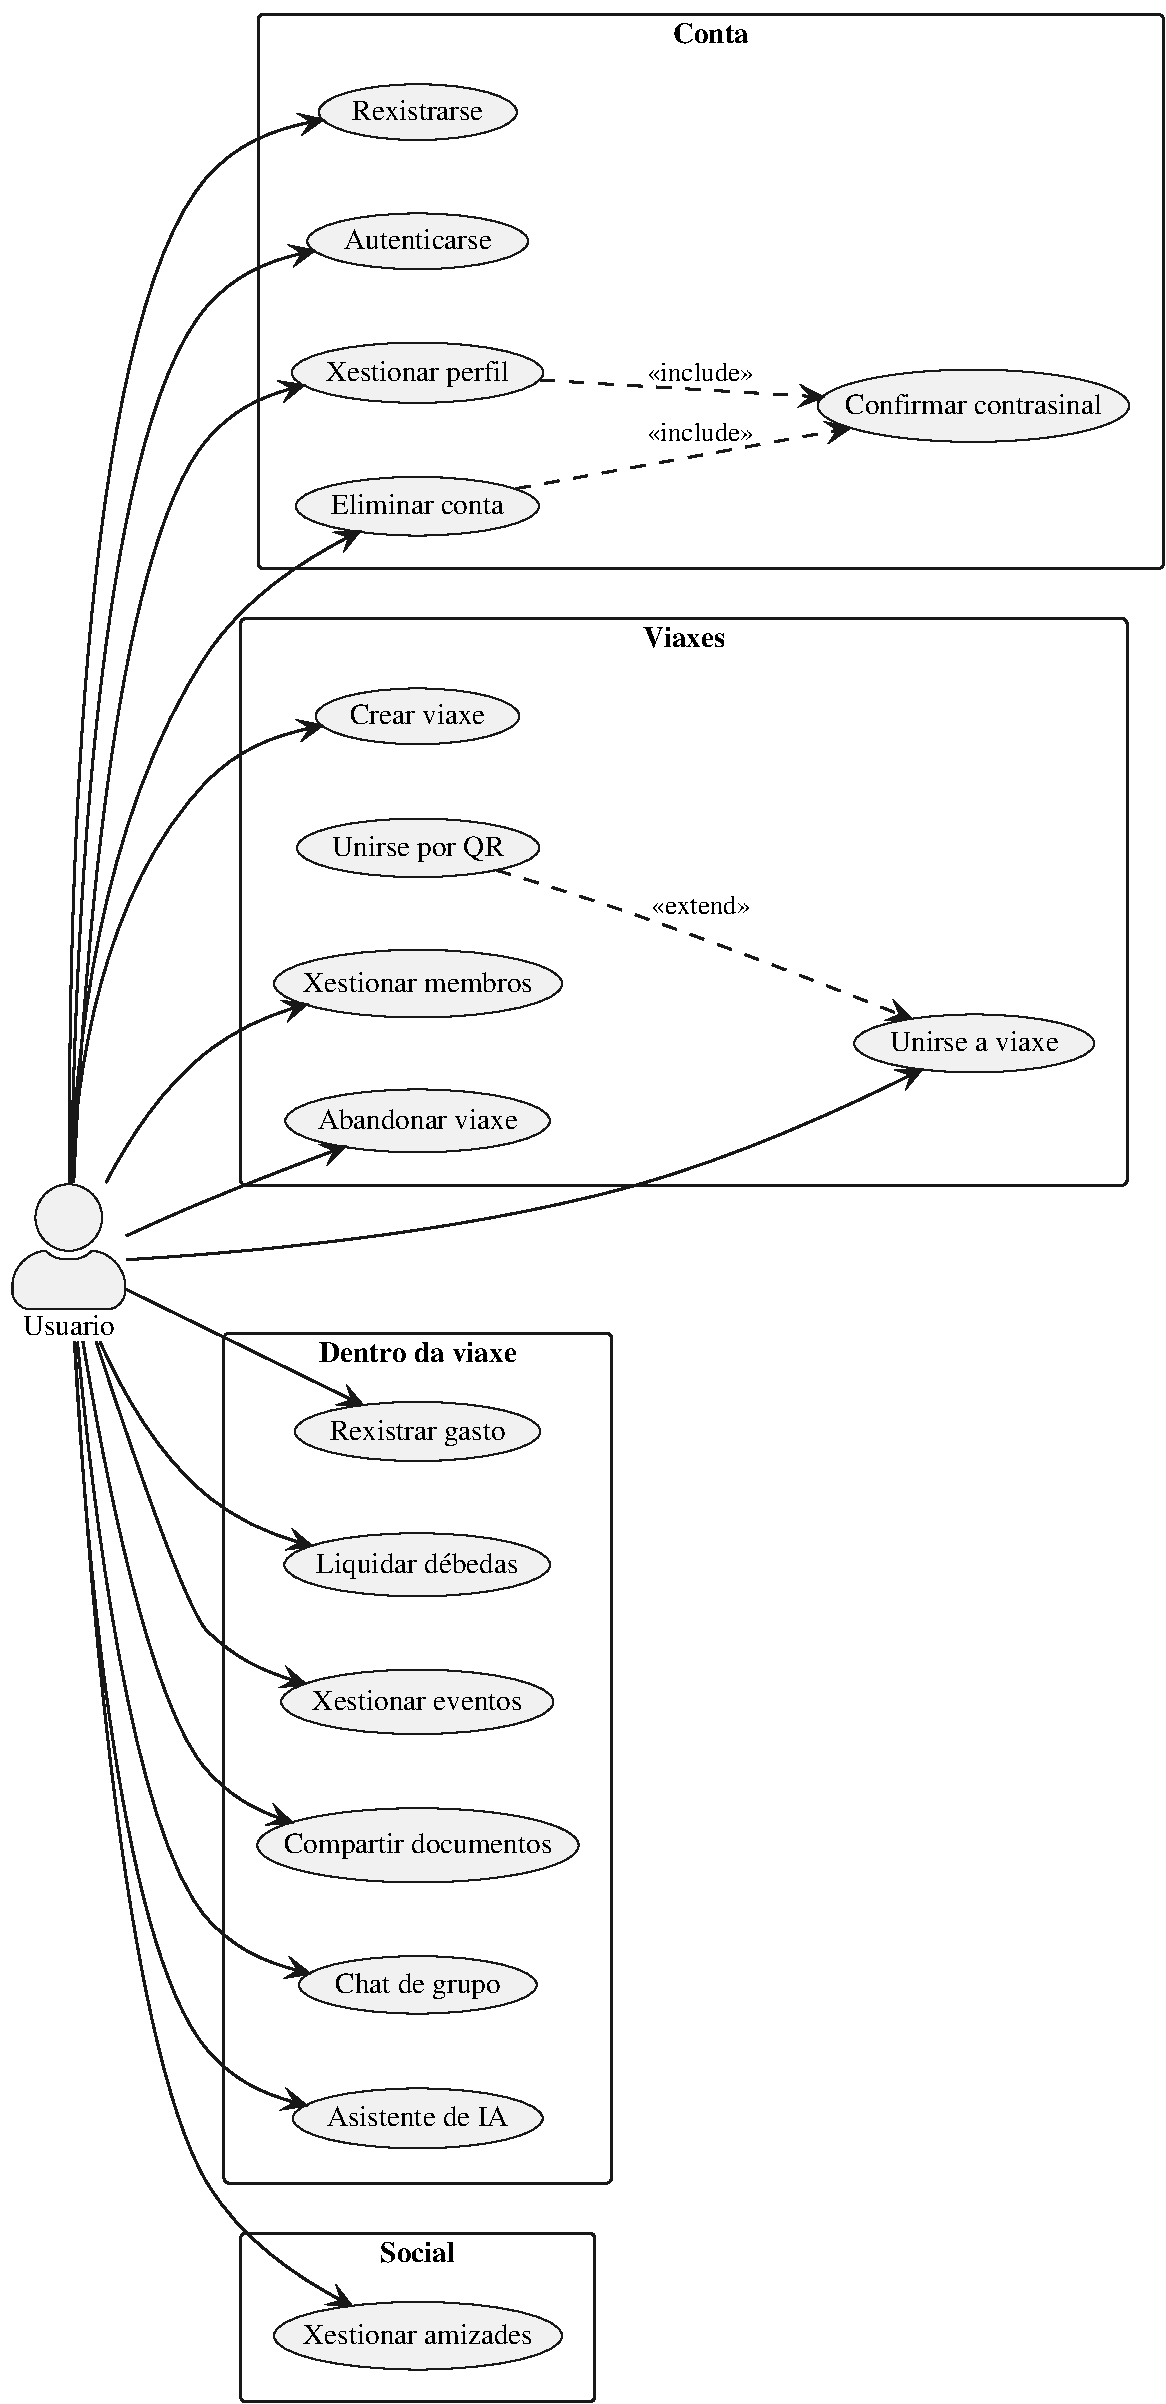
\includegraphics[width=0.52\textwidth]{diagrams/casos-uso.pdf}
  \caption{Diagrama de casos de uso de Telaria (actor único: Usuario).}
  \label{fig:casos-uso}
\end{figure}

\paragraph*{CU01. Rexistro e autenticación.}
\begin{itemize}[noitemsep,topsep=2pt]
  \item \textbf{Actor:} Usuario.
  \item \textbf{Precondicións:} dispón da aplicación instalada e de conexión á rede.
  \item \textbf{Fluxo principal:} (1) introduce nome de usuario, correo e contrasinal e solicita o rexistro; (2) o sistema crea a conta, almacena o contrasinal cifrado e devolve un \textit{access token} JWT e un \textit{refresh token}; (3) o usuario queda autenticado. O inicio de sesión posterior realízase con correo e contrasinal.
  \item \textbf{Fluxos alternativos:} correo xa rexistrado $\rightarrow$ o sistema rexeita o rexistro; credenciais incorrectas no inicio de sesión $\rightarrow$ erro de autenticación; caducidade do \textit{access token} $\rightarrow$ o cliente renóvao de forma transparente co \textit{refresh token}.
  \item \textbf{Poscondición:} o usuario dispón dunha sesión activa.
  \item \textbf{Requisitos:} RF01, RF02.
\end{itemize}

\paragraph*{CU02. Unirse a unha viaxe.}
\begin{itemize}[noitemsep,topsep=2pt]
  \item \textbf{Actor:} Usuario.
  \item \textbf{Precondicións:} usuario autenticado.
  \item \textbf{Fluxo principal (por invitación):} (1) un membro da viaxe convída ao usuario; (2) o usuario recibe a notificación e acepta a invitación; (3) o sistema rexistra a adhesión e o usuario pasa a ser membro da viaxe.
  \item \textbf{Fluxos alternativos:} por solicitude (o usuario solicita unirse a partir dun identificador de viaxe e calquera membro aproba a solicitude); por QR (o usuario escanea un código QR que o sistema procesa como invitación directa).
  \item \textbf{Poscondición:} o usuario figura na lista de membros da viaxe.
  \item \textbf{Requisitos:} RF07, RF08.
\end{itemize}

\paragraph*{CU03. Rexistrar un gasto e liquidar débedas.}
\begin{itemize}[noitemsep,topsep=2pt]
  \item \textbf{Actor:} Usuario (membro da viaxe).
  \item \textbf{Precondicións:} o usuario é membro da viaxe.
  \item \textbf{Fluxo principal:} (1) rexistra un gasto (importe, nome, categoría, pagador e beneficiarios); (2) o sistema garda o gasto e recalcula os balances; (3) o membro consulta quen debe a quen; (4) cando se salda unha débeda, rexístrase a liquidación correspondente.
  \item \textbf{Fluxos alternativos:} o pagador ou algún beneficiario non é membro da viaxe $\rightarrow$ erro de validación.
  \item \textbf{Poscondición:} os balances reflicten o novo gasto; as liquidacións rexistradas reducen as débedas pendentes.
  \item \textbf{Requisitos:} RF10, RF11.
\end{itemize}

\paragraph*{CU04. Xestionar os membros da viaxe.}
\begin{itemize}[noitemsep,topsep=2pt]
  \item \textbf{Actor:} Usuario (membro da viaxe).
  \item \textbf{Precondicións:} o usuario é membro da viaxe.
  \item \textbf{Fluxo principal:} (1) convida a outro usuario (por identificador, amizade ou QR) ou consulta as solicitudes de unión pendentes; (2) acepta ou rexeita unha solicitude; (3) o sistema actualiza a lista de membros.
  \item \textbf{Fluxos alternativos:} usuario xa membro ou xa convidado $\rightarrow$ conflito.
  \item \textbf{Poscondición:} a composición da viaxe queda actualizada. Calquera membro pode realizar estas accións: non hai roles.
  \item \textbf{Requisitos:} RF08, RF17.
\end{itemize}

\paragraph*{CU05. Subir un documento.}
\begin{itemize}[noitemsep,topsep=2pt]
  \item \textbf{Actor:} Usuario (membro da viaxe).
  \item \textbf{Precondicións:} o usuario é membro da viaxe.
  \item \textbf{Fluxo principal:} (1) inicia a subida indicando nome e tipo de contido; (2) o sistema crea o rexistro e devolve unha URL prefirmada; (3) o cliente sobe o ficheiro directamente ao almacén de obxectos; (4) o cliente confirma a subida e o sistema marca o documento como dispoñible, xerando unha miniatura de forma asíncrona se é unha imaxe.
  \item \textbf{Fluxos alternativos:} se a subida non se confirma, unha tarefa programada verifica a existencia do arquivo no almacenamento e, de existir, a marca como confirmada; en caso contrario, elimina o rexistro orfo.
  \item \textbf{Poscondición:} o documento queda listado e descargable mediante URL prefirmada.
  \item \textbf{Requisitos:} RF13.
\end{itemize}

\paragraph*{CU06. Eliminar a conta.}
\begin{itemize}[noitemsep,topsep=2pt]
  \item \textbf{Actor:} Usuario.
  \item \textbf{Precondicións:} usuario autenticado.
  \item \textbf{Fluxo principal:} (1) solicita eliminar a súa conta; (2) o sistema solicita a confirmación do contrasinal; (3) tras a verificación, elimínanse os datos persoais e os artefactos asociados (avatares, documentos) e retírase o usuario das viaxes compartidas; (4) péchase a sesión.
  \item \textbf{Fluxos alternativos:} contrasinal incorrecto $\rightarrow$ cancélase a operación.
  \item \textbf{Poscondición:} a conta e os datos persoais quedan eliminados.
  \item \textbf{Requisitos:} RF03, RF04.
\end{itemize}

% -----------------------------------------------------------------------
\section{Requisitos non funcionais}

\subsection{Seguridade}

\begin{itemize}
  \item \textbf{RNF-SE-01}. Control de acceso: só os membros dunha viaxe acceden aos seus datos; calquera usuario autenticado pode crear viaxes.
  \item \textbf{RNF-SE-02}. Os contrasinais almacénanse con hash BCrypt; os \textit{access tokens} JWT teñen vida curta e os \textit{refresh tokens} opacos almacénanse no servidor para limitar a exposición ante intrusións.
  \item \textbf{RNF-SE-03}. As operacións sensibles sobre a conta (o cambio de correo electrónico e a eliminación da conta) requiren a confirmación do contrasinal actual.
\end{itemize}

\subsection{Privacidade e protección de datos}

\begin{itemize}
  \item \textbf{RNF-PR-01}. A eliminación da conta borra os datos persoais do usuario e os artefactos asociados no almacén de obxectos (avatar e documentos), e retírao das viaxes compartidas.
  \item \textbf{RNF-PR-02}. As mensaxes de chat (de grupo e do asistente de IA) elimínanse automaticamente tras un período de retención de 30 días mediante unha tarefa programada.
\end{itemize}

\subsection{Rendemento}

\begin{itemize}
  \item \textbf{RNF-RE-01}. O cálculo de liquidacións realízase no servidor, evitando sobrecargar o dispositivo cliente.
  \item \textbf{RNF-RE-02}. A entrega de mensaxes do chat e das respostas do asistente de IA realízase en tempo real mediante eventos enviados polo servidor (SSE).
  \item \textbf{RNF-RE-03}. A xeración de miniaturas dos documentos de imaxe execútase de forma asíncrona, fóra da ruta de petición, para non penalizar a latencia da subida nin da listaxe.
\end{itemize}

\subsection{Usabilidade}

\begin{itemize}
  \item \textbf{RNF-US-01}. A interface debe ser intuitiva e usable sen formación previa.
  \item \textbf{RNF-US-02}. A aplicación estará dispoñible en galego, castelán e inglés.
  \item \textbf{RNF-US-03}. A aplicación proporcionará retroalimentación visual inmediata
        ante cada acción relevante (indicadores de carga, confirmacións e mensaxes de erro),
        conforme ao heurístico de visibilidade do estado do sistema de Nielsen.
  \item \textbf{RNF-US-04}. A interface será consistente en terminoloxía, iconas e
        comportamento en todas as pantallas, seguindo o heurístico de coherencia e estándares
        de Nielsen.
  \item \textbf{RNF-US-05}. A paleta de cores respectará os estándares de accesibilidade:
        a información crítica non dependerá unicamente da cor, de xeito que sexa interpretable
        por usuarios con déficit de percepción cromática.
\end{itemize}

\subsection{Mantibilidade}

\begin{itemize}
  \item \textbf{RNF-MA-01}. O contrato OpenAPI é a fonte de verdade da API: a partir del xéranse automaticamente as interfaces e DTO do backend e os tipos do frontend, garantindo a sincronía entre ambos os extremos.
  \item \textbf{RNF-MA-02}. A lóxica do backend está cuberta por unha batería de probas automatizadas (unitarias e de integración) que facilita a evolución segura do código.
\end{itemize}

\subsection{Portabilidade e despregamento}

\begin{itemize}
  \item \textbf{RNF-PO-01}. O backend e os servizos auxiliares despreganse en contedores Podman.
  \item \textbf{RNF-PO-02}. A aplicación móbil é compatible con iOS e Android mediante Expo/React Native.
\end{itemize}

\subsection{Interoperabilidade}

\begin{itemize}
  \item \textbf{RNF-IN-01}. O almacenamento de documentos baséase no protocolo estándar S3, o que garante a independencia respecto dun provedor concreto.
\end{itemize}

\subsection{Fiabilidade}

\begin{itemize}
  \item \textbf{RNF-FI-01}. O sistema valida os datos de entrada na API e devolve mensaxes de erro claras e estruturadas ao cliente.
  \item \textbf{RNF-FI-02}. Unha tarefa programada reconcilia periodicamente as subidas de documentos non confirmadas (orfas): confirma as que efectivamente existen no almacén de obxectos e elimina os rexistros sen ficheiro asociado, evitando entradas inconsistentes na base de datos.
\end{itemize}

% -----------------------------------------------------------------------
\section{Información que o sistema debe almacenar}

A persistencia do sistema repártese en tres niveis complementarios segundo a natureza do
dato. A información estruturada do dominio (usuarios, viaxes, eventos, gastos, mensaxes,
etc.) almacénase nunha base de datos relacional \textbf{PostgreSQL}, onde Hibernate mapea
cada entidade á súa táboa. Os \textbf{ficheiros binarios} (documentos compartidos e
avatares) non se gardan na base de datos, senón nun \textbf{almacén de obxectos}. Por
último, o dispositivo do usuario conserva localmente un pequeno conxunto de datos de
sesión e de preferencias que se detalla máis adiante. O Cadro~\ref{tab:entidades} recolle
as principais entidades persistidas no servidor e os seus atributos.

\begin{longtable}{@{}p{4cm}p{10.3cm}@{}}
  \caption{Entidades persistidas no servidor.}
  \label{tab:entidades} \\
  \toprule
  \textbf{Entidade} & \textbf{Atributos principais} \\
  \midrule
  \endfirsthead
  \caption*{Cadro~\ref{tab:entidades} (continuación)} \\
  \toprule
  \textbf{Entidade} & \textbf{Atributos principais} \\
  \midrule
  \endhead
  Usuario                    & Identificador (UUID), nome de usuario, correo electrónico, contrasinal (hash). \\[4pt]
  Viaxe                      & Identificador (UUID), nome, data de creación, conxunto de membros (usuarios). \\[4pt]
  Evento                     & Identificador, nome, data e hora de inicio (con fuso horario), duración en minutos, localización embebida (nome, enderezo, latitude, lonxitude). \\[4pt]
  Gasto                      & Identificador, importe (decimal), nome, categoría (enumeración), usuario pagador, usuario creador do rexistro, conxunto de beneficiarios, marca temporal. \\[4pt]
  Liquidación                & Identificador, importe (decimal), usuario pagador, usuario receptor, marca temporal. \\[4pt]
  Documento compartido       & Identificador, nome de ficheiro, clave no almacén de obxectos, clave da miniatura de previsualización, estado de subida (booleano), usuario creador, marca temporal. \\[4pt]
  Invitación / Solicitude    & Identificador, usuario, viaxe asociada, marca temporal de creación. \\[4pt]
  Amizade                    & Identificador (UUID), dous usuarios asociados (almacenados de forma normalizada para garantir a unicidade da parella), marca temporal de creación. \\[4pt]
  Solicitude de amizade      & Identificador (UUID), usuario emisor, usuario receptor, marca temporal de creación. \\[4pt]
  Mensaxe de chat de grupo   & Identificador, contido (texto), autor, viaxe asociada, marca temporal. \\[4pt]
  Mensaxe de asistente de IA & Identificador, contido (texto), rol (USUARIO ou ASISTENTE), usuario, viaxe asociada, marca temporal. \\[4pt]
  Token de refresco          & Token (identificador), identificador do usuario asociado. \\
  \bottomrule
\end{longtable}

\subsection{Almacenamento de ficheiros (MinIO)}

Os ficheiros que sobe o usuario (documentos compartidos das viaxes e imaxes de avatar)
non son axeitados para gardarse nunha base de datos relacional: trátase de obxectos
binarios potencialmente grandes que cargarían as táboas, dificultarían as copias de
seguranza e penalizarían o rendemento das consultas. Por iso o sistema delega a súa
custodia nun \textbf{almacén de obxectos compatible coa API de Amazon~S3}, para o que se
emprega \textbf{MinIO}, unha solución de código aberto. A vantaxe de MinIO é que é
\textbf{autoxestionado}: en lugar de contratar un servizo de almacenamento na nube como
Amazon~S3 (onde os ficheiros residen na infraestrutura dun provedor externo e o seu uso se
factura por consumo), MinIO execútase na propia infraestrutura do proxecto, despregándose
de xeito sinxelo como un contedor (Docker / Podman) xunto co resto de servizos. Isto
elimina a dependencia e os custos dun provedor comercial e, ao expoñer a mesma API que
S3, permitiría migrar a ese servizo no futuro sen apenas cambios no código.

A base de datos non garda o contido do ficheiro, senón unicamente os \textbf{metadatos}
necesarios para localizalo: a clave do obxecto dentro do almacén (\textit{object key}), a
clave da miniatura de previsualización e o estado da subida. Deste xeito mantense unha
única fonte de verdade (o rexistro relacional referencia o obxecto físico) e evítase a
duplicación de datos pesados.

A interacción co almacén realízase mediante \textbf{URLs prefirmadas}: cando un usuario
quere subir ou descargar un ficheiro, o backend xera unha URL temporal e asinada que
autoriza esa operación concreta durante un período limitado. O cliente comunícase
\textbf{directamente} con MinIO empregando esa URL, polo que o servidor de aplicación
nunca chega a recibir nin a servir os bytes do ficheiro. Esta arquitectura descarga o
backend, mellora a escalabilidade e reduce a latencia das transferencias.

\subsection{Información almacenada no dispositivo (frontend)}

Ademais da persistencia no servidor, a aplicación móbil garda localmente no dispositivo un
conxunto reducido de información para soster a sesión entre execucións e recordar as
preferencias da persoa usuaria. As credenciais de sesión (os \textit{tokens}) gárdanse no
\textbf{almacén seguro e cifrado do sistema operativo}, respaldado pola \textit{keychain}
de iOS ou o \textit{keystore} de Android, mentres que o resto de valores, ao non ser
sensibles, se persisten no almacenamento clave-valor convencional do dispositivo. O
Cadro~\ref{tab:frontend-storage} resume o que se garda no cliente.

\begin{longtable}{@{}p{3.6cm}p{10.7cm}@{}}
  \caption{Datos persistidos localmente no dispositivo do cliente.}
  \label{tab:frontend-storage} \\
  \toprule
  \textbf{Clave} & \textbf{Contido e propósito} \\
  \midrule
  \endfirsthead
  \toprule
  \textbf{Clave} & \textbf{Contido e propósito} \\
  \midrule
  \endhead
  \texttt{refreshToken} & Token de refresco da sesión (cifrado); permite obter novos tokens de acceso sen volver iniciar sesión. \\[3pt]
  \texttt{accessToken}  & Token de acceso vixente (cifrado) que autoriza as peticións á API. \\[3pt]
  \texttt{userEmail}    & Correo electrónico da persoa usuaria autenticada. \\[3pt]
  \texttt{username}     & Nome de usuario mostrado na interface. \\[3pt]
  \texttt{app\_language} & Idioma escollido para a interface (es / en / gl). \\[3pt]
  \texttt{app\_theme}    & Tema visual seleccionado (claro / escuro). \\[3pt]
  \texttt{app\_data\_saver} & Indicador do modo de aforro de datos. \\[3pt]
  \texttt{lastTripId}   & Identificador da última viaxe aberta, para restaurar a navegación. \\[3pt]
  \texttt{lastTripTab}  & Última pestana visitada dentro dunha viaxe. \\
  \bottomrule
\end{longtable}

Este almacenamento local é deliberadamente mínimo: non se replica no dispositivo o
contido das viaxes nin datos doutros usuarios, senón unicamente o estritamente preciso
para reanudar a sesión e personalizar a experiencia. Ao pechar sesión, tanto as
credenciais cifradas como o estado de navegación bórranse do dispositivo.

\chapter{Deseño}

Neste capítulo descríbese como se constrúe o sistema: a súa arquitectura xeral, a
división en compoñentes e a comunicación entre eles, o modelo de datos, o deseño da API
e dos extremos cliente e servidor, os fluxos máis relevantes e, por último, o
equipamento hardware e software empregado. Sempre que é posible recórrese a
representacións gráficas para facilitar a comprensión da estrutura do produto.

\section{Arquitectura xeral do sistema}

Telaria segue unha arquitectura \textbf{cliente–servidor} de tres capas lóxicas
(presentación, lóxica de negocio e persistencia) e adopta un enfoque \textit{API-first}:
o contrato da API, especificado con OpenAPI, é o punto de partida do desenvolvemento e o
elemento que vincula o cliente co servidor. A Figura~\ref{fig:arquitectura} mostra a
visión de conxunto.

\begin{figure}[H]
  \centering
  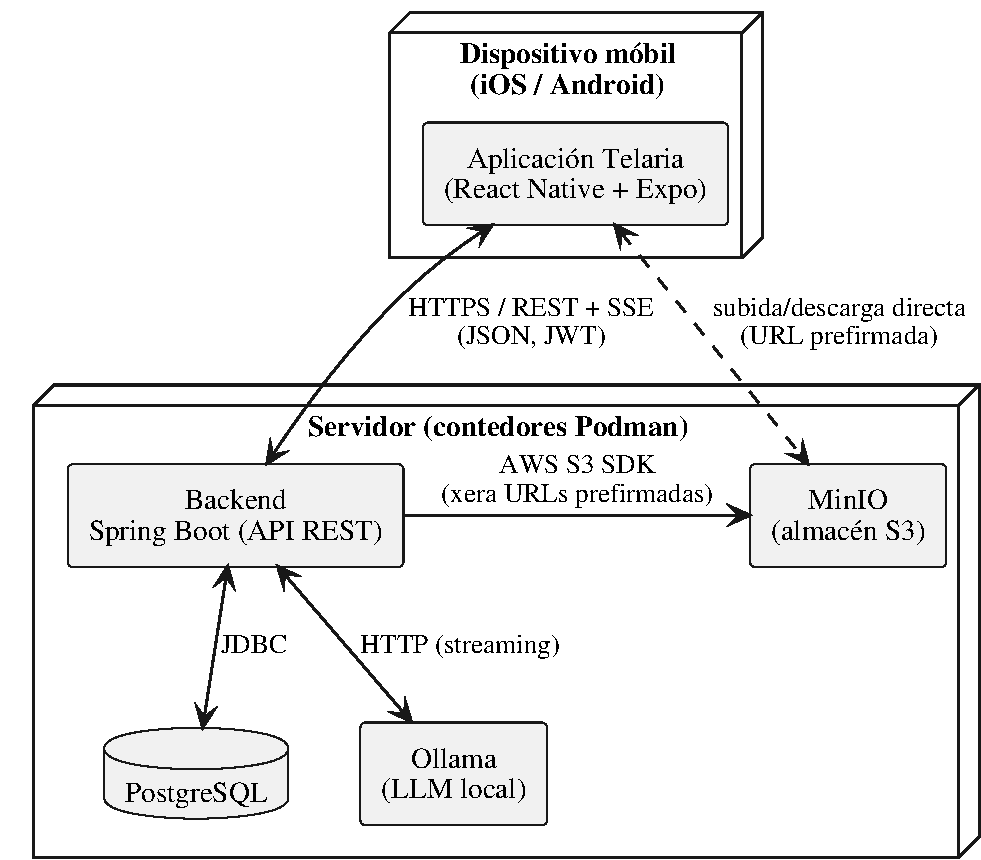
\includegraphics[width=0.72\textwidth]{diagrams/arquitectura.pdf}
  \caption{Arquitectura xeral e despregamento de Telaria.}
  \label{fig:arquitectura}
\end{figure}

O \textbf{cliente} é unha aplicación móbil multiplataforma (React Native + Expo) que se
executa en iOS e Android. O \textbf{servidor} agrupa, en contedores xestionados con
Podman, o backend Spring Boot e os tres servizos de apoio: a base de datos PostgreSQL, o
almacén de obxectos compatible con S3 (MinIO) e o motor de inferencia de modelos de
linguaxe (Ollama).

A comunicación principal entre cliente e servidor realízase sobre HTTP mediante unha API
REST que intercambia JSON e protexe cada petición cun \textit{access token} JWT. Para as
funcionalidades en tempo real (chat de grupo e asistente de IA), o servidor emprega
\textit{Server-Sent Events} (SSE), que permiten un fluxo unidireccional de eventos do
servidor cara ao cliente sobre a mesma conexión HTTP. Finalmente, a subida e a descarga
de documentos non pasan polo backend: este limítase a xerar \textit{URLs prefirmadas} co
que o cliente fala \textbf{directamente} co almacén de obxectos, descargando o servidor
da transferencia de ficheiros.

\section{Arquitectura do backend}

O backend organízase nunha arquitectura por capas que separa claramente as
responsabilidades, como se aprecia na Figura~\ref{fig:backend}.

\begin{figure}[H]
  \centering
  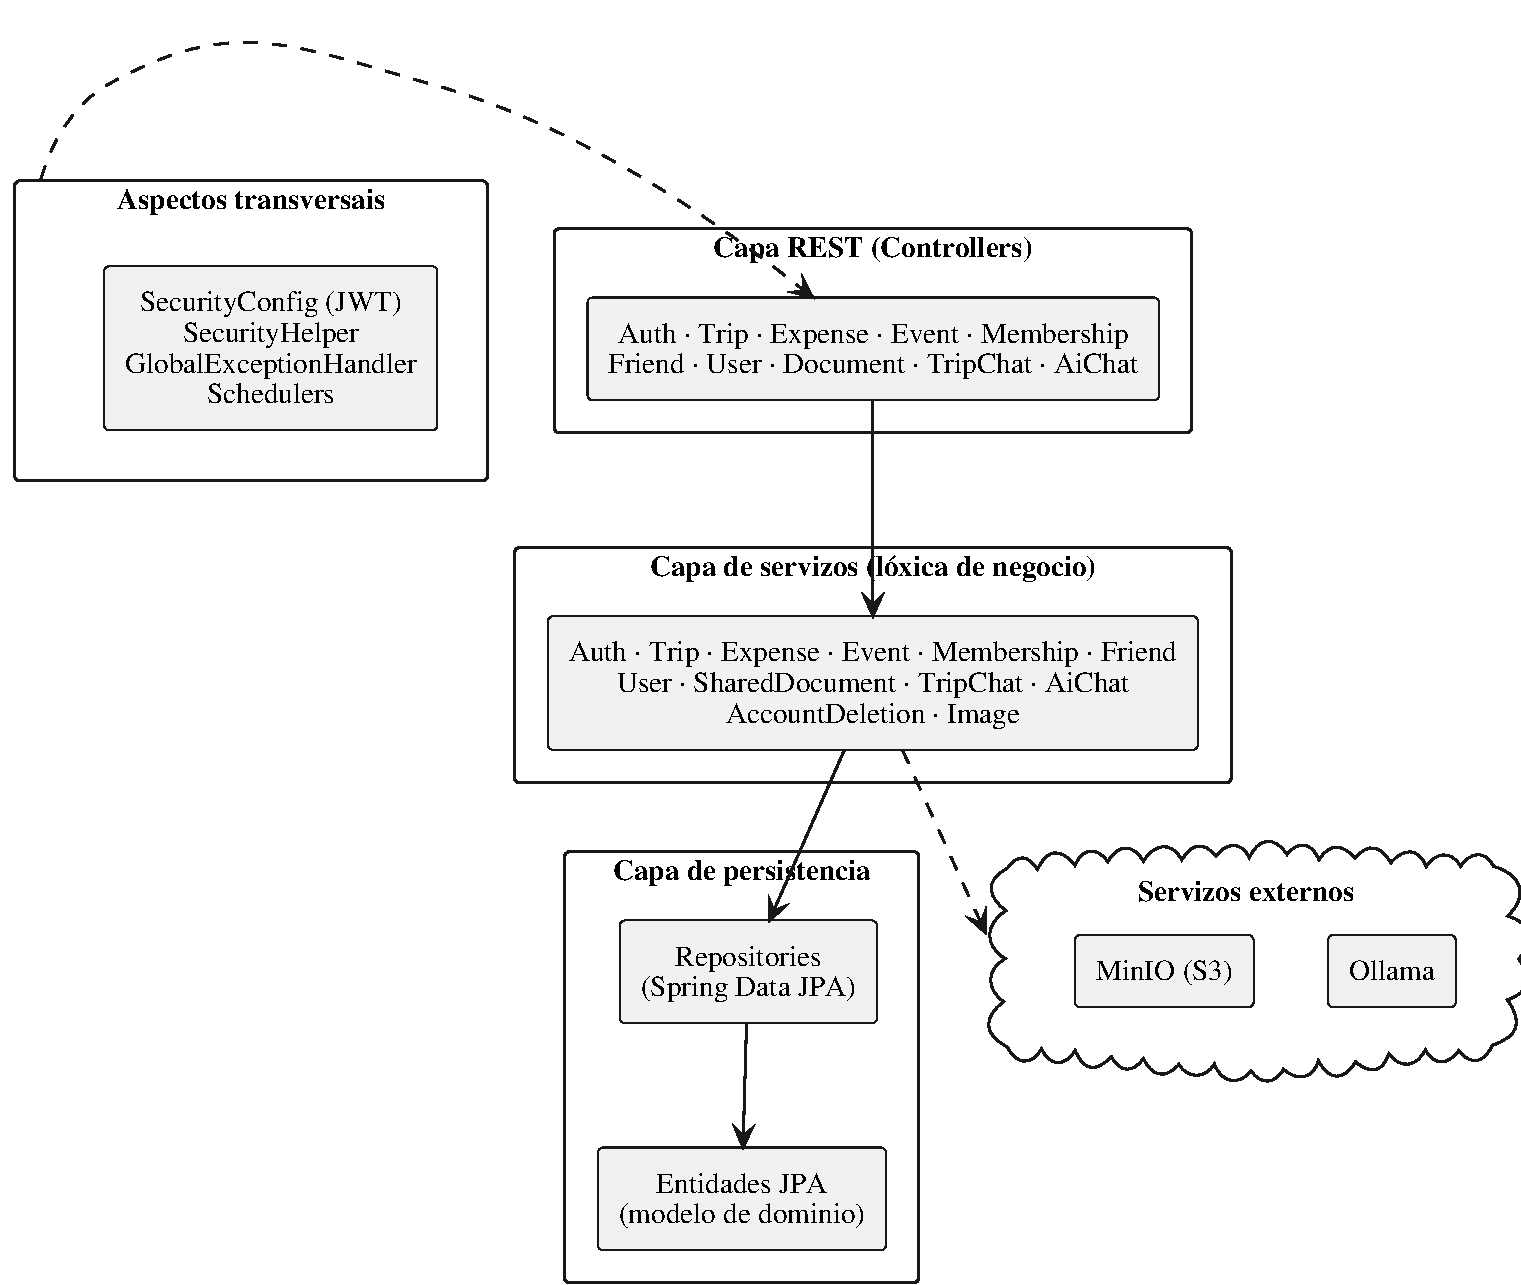
\includegraphics[width=0.85\textwidth]{diagrams/backend-componentes.pdf}
  \caption{Compoñentes e capas do backend.}
  \label{fig:backend}
\end{figure}

\begin{itemize}
  \item \textbf{Capa REST (controllers).} Expón os \textit{endpoints} da API. As
        interfaces destes controladores xéranse automaticamente a partir do contrato
        OpenAPI, e as clases que as implementan conteñen unicamente a tradución entre a
        petición HTTP e a chamada ao servizo correspondente.
  \item \textbf{Capa de servizos.} Concentra a lóxica de negocio: validacións,
        cálculo de liquidacións, resolución de invitacións e solicitudes, xestión de
        ficheiros, etc. É a única capa que coordina varias entidades e repositorios
        dentro dunha mesma transacción.
  \item \textbf{Capa de persistencia.} Componse dos repositorios de Spring Data JPA e
        das entidades do modelo de dominio, que Hibernate mapea ás táboas de PostgreSQL.
  \item \textbf{Aspectos transversais.} A configuración de seguridade (validación de
        tokens JWT con Spring Security), a utilidade de extracción do usuario autenticado
        (\texttt{SecurityHelper}), o manexo centralizado de erros
        (\texttt{GlobalExceptionHandler}, que devolve respostas no formato
        \textit{Problem Details}, RFC~7807)~\cite{rfc7807} e as tarefas programadas
        (\textit{schedulers}) de limpeza e xeración de miniaturas.
\end{itemize}

A autorización aplícase na capa de servizos: o acceso aos datos dunha viaxe verifícase
comprobando que o usuario autenticado pertence aos seus membros, de modo que ningún
usuario poida acceder á información de viaxes das que non forma parte.

\section{Modelo de datos}

A Figura~\ref{fig:modelo} representa o modelo de dominio coas entidades persistentes e as
súas relacións.

\begin{figure}[H]
  \centering
  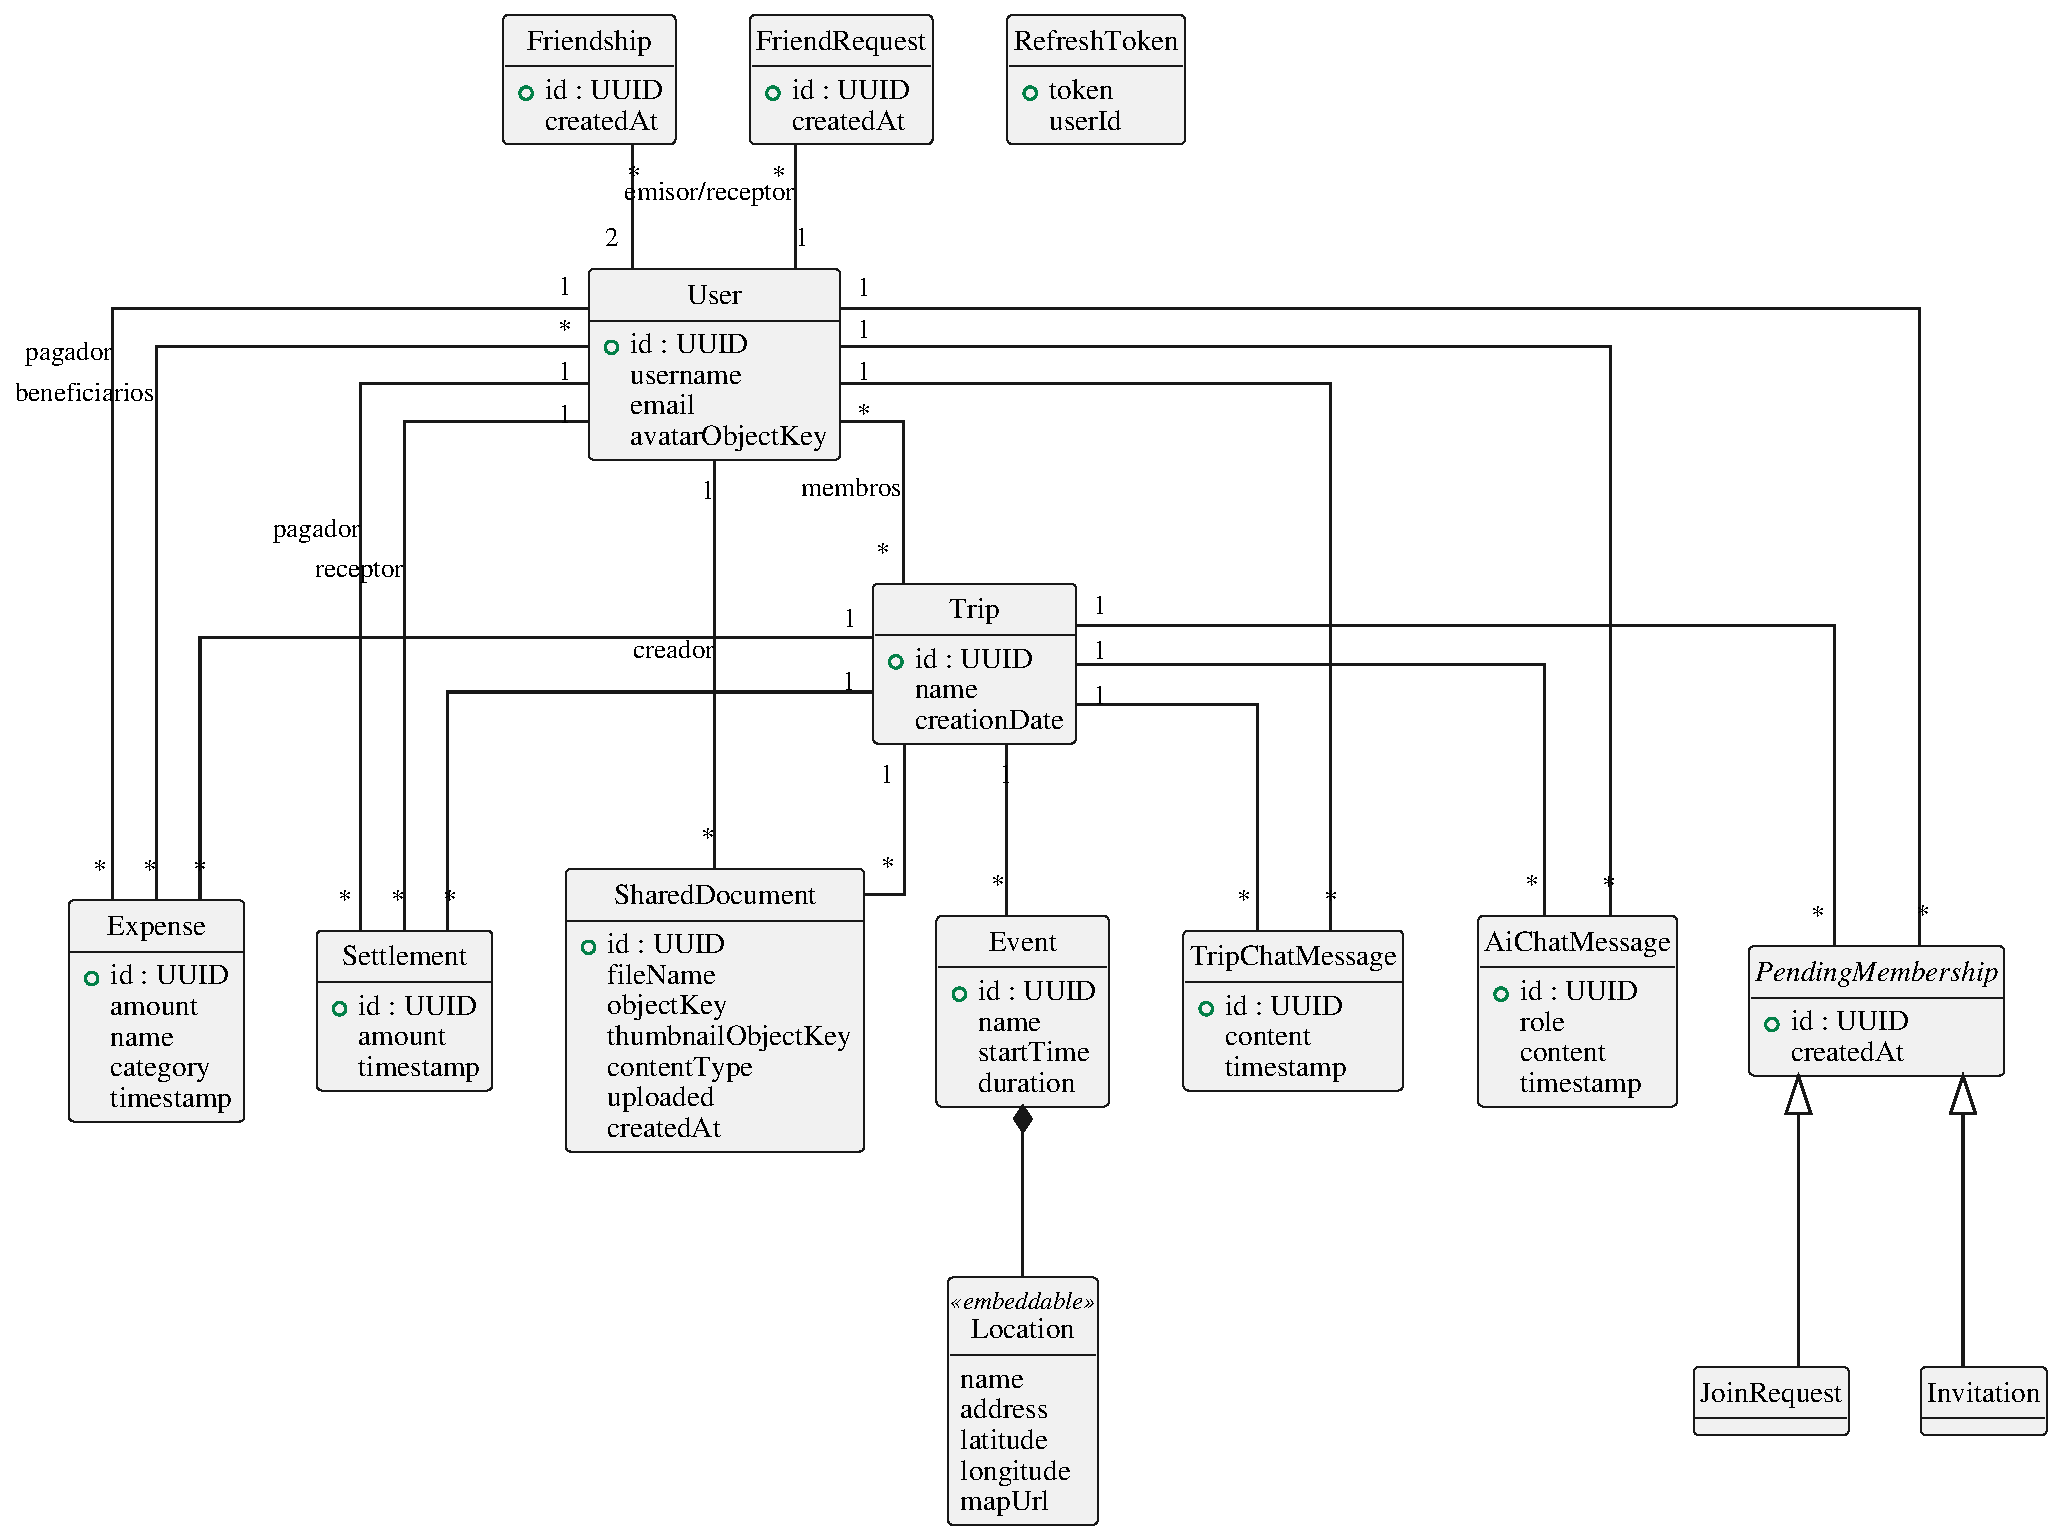
\includegraphics[width=\textwidth]{diagrams/modelo-datos.pdf}
  \caption{Modelo de datos (entidades e relacións principais).}
  \label{fig:modelo}
\end{figure}

As decisións de deseño máis salientables son:

\begin{itemize}
  \item \textbf{Identificadores UUID.} Todas as entidades principais empregan UUID como
        clave primaria, o que evita expor identificadores secuenciais e facilita a
        xeración de claves no lado da aplicación.
  \item \textbf{Relacións varios-a-varios.} A pertenza ás viaxes
        (\texttt{User}\,--\,\texttt{Trip}) e os beneficiarios dun gasto
        (\texttt{Expense}\,--\,\texttt{User}) modélanse mediante táboas de unión.
  \item \textbf{Normalización das amizades.} Cada \texttt{Friendship} almacena os dous
        usuarios de forma ordenada (o de identificador menor primeiro), o que garante a
        unicidade da parella e simplifica as consultas bidireccionais.
  \item \textbf{Valor embebido.} A localización dun evento (\texttt{Location}: nome,
        enderezo, coordenadas e URL de mapa) modélase como un obxecto embebido dentro de
        \texttt{Event}, ao non ter identidade propia (considérase que os diferentes eventos
         non compartirán ubicación frecuentemente).
  \item \textbf{Xerarquía de membros pendentes.} \texttt{Invitation} e
        \texttt{JoinRequest} comparten estrutura (viaxe, usuario e marca temporal) a
        través da superclase \texttt{PendingMembership}, diferenciándose só na
        dirección da petición.
  \item \textbf{Token de refresco persistente.} O \texttt{RefreshToken} almacénase no
        servidor para poder invalidalo no peche de sesión.
\end{itemize}

O esquema da base de datos non se xestiona con ferramentas de migración: emprégase a
xeración automática de Hibernate (\texttt{ddl-auto}), apropiada para o contexto deste
proxecto. Na sección de conclusións recóllese a adopción de migracións explícitas como
posible mellora de cara a un entorno de produción.

\section{Deseño da API REST}

A API é o contrato central do sistema e especifícase con \textbf{OpenAPI} de forma
modular: un documento principal (\texttt{api.yaml}) referencia, mediante \texttt{\$ref},
ficheiros independentes para as rutas (\texttt{paths/}) e para os esquemas de datos
(\texttt{schemas/}). Esta organización mantén o contrato lexible malia o seu tamaño.

A partir deste contrato xérase código automaticamente en ambos os extremos:

\begin{itemize}
  \item No \textbf{backend}, o complemento \textit{OpenAPI Generator} produce as
        interfaces dos controladores e os obxectos de transferencia de datos (DTO).
  \item No \textbf{frontend}, a ferramenta \texttt{openapi-typescript} xera os tipos
        TypeScript que describen as peticións e respostas.
\end{itemize}

Deste xeito, calquera cambio no contrato propágase automaticamente como tipos a ambos os
extremos, e calquera incoherencia detéctase en tempo de compilación. Ademais, a partir
da mesma especificación ofrécese documentación interactiva da API (Swagger UI). A
Táboa~\ref{tab:recursos} resume os principais recursos da API.

\begin{table}[H]
  \centering
  \begin{tabularx}{\textwidth}{@{}lX@{}}
    \toprule
    \textbf{Recurso} & \textbf{Responsabilidade} \\
    \midrule
    \texttt{/auth}                    & Rexistro, inicio e peche de sesión, renovación de tokens. \\
    \texttt{/users}                   & Perfil, contrasinal, avatar, eliminación de conta. \\
    \texttt{/trips}                   & Creación e consulta de viaxes. \\
    \texttt{/trips/[tripID]/expenses}      & Gastos, balances e liquidacións. \\
    \texttt{/trips/[tripID]/events}        & Eventos do calendario. \\
    \texttt{/trips/[tripID]/documents}     & Documentos compartidos (subida en varios pasos). \\
    \texttt{/trips/[tripID]/group-chat}    & Chat de grupo (consulta, envío e fluxo SSE). \\
    \texttt{/trips/[tripID]/ai-chat}       & Asistente de IA (historial e resposta en \textit{streaming}). \\
    Invitacións, solicitudes, amizades & Xestión de membros e da rede social de usuarios. \\
    \bottomrule
  \end{tabularx}
  \caption{Resumo dos principais recursos da API REST.}
  \label{tab:recursos}
\end{table}

\section{Arquitectura do frontend}

O cliente organízase tamén por capas, como amosa a
Figura~\ref{fig:frontend}. A navegación baséase en \textbf{Expo Router}, un sistema de
rutas baseado na estrutura de ficheiros, que agrupa as pantallas en tres grupos
(\texttt{(auth)}, \texttt{(main)} e \texttt{(trip)}).

\begin{figure}[H]
  \centering
  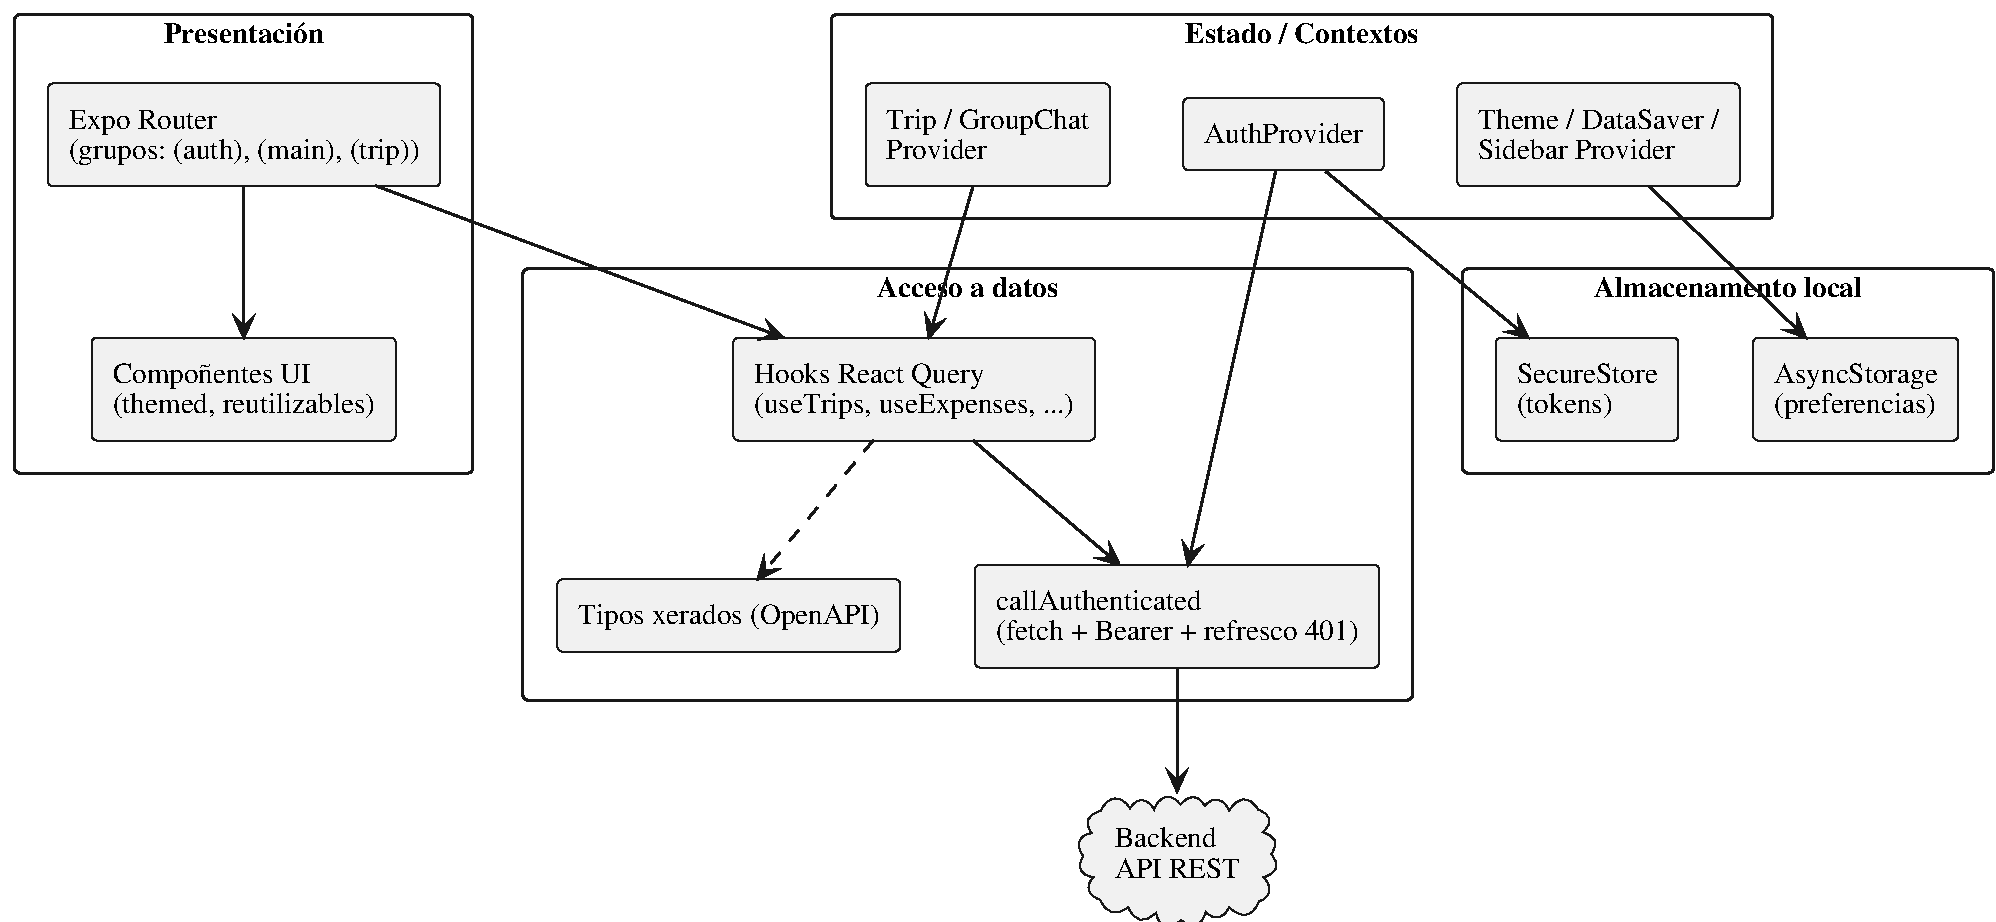
\includegraphics[width=\textwidth]{diagrams/frontend-arquitectura.pdf}
  \caption{Arquitectura do frontend.}
  \label{fig:frontend}
\end{figure}

O estado da aplicación divídese en dous tipos. O \textbf{estado de servidor} (datos que
proveñen do backend) xestiónase con \textbf{React Query}~\cite{reactquery}, que se encarga da caché, da
revalidación e da sincronización; cada recurso ten os seus \textit{hooks} de consulta e
mutación e unha factoría de claves de caché. O \textbf{estado de aplicación} (sesión,
tema, viaxe actual, chat) maniféstase mediante contextos de React
(\texttt{AuthProvider}, \texttt{ThemeProvider}, \texttt{TripProvider},
\texttt{GroupChatProvider}, etc.).

Toda chamada autenticada pasa por unha función envoltorio
(\texttt{callAuthenticated}) que engade o \textit{access token} á cabeceira
\texttt{Authorization} e, ante unha resposta \texttt{401}, renova o token de forma
transparente e reintenta a petición. Os tokens gárdanse de forma cifrada
(\texttt{SecureStore}) e as preferencias do usuario en almacenamento local
(\texttt{AsyncStorage}). A Figura~\ref{fig:navegacion} mostra o mapa completo de
navegación.

\begin{figure}[H]
  \centering
  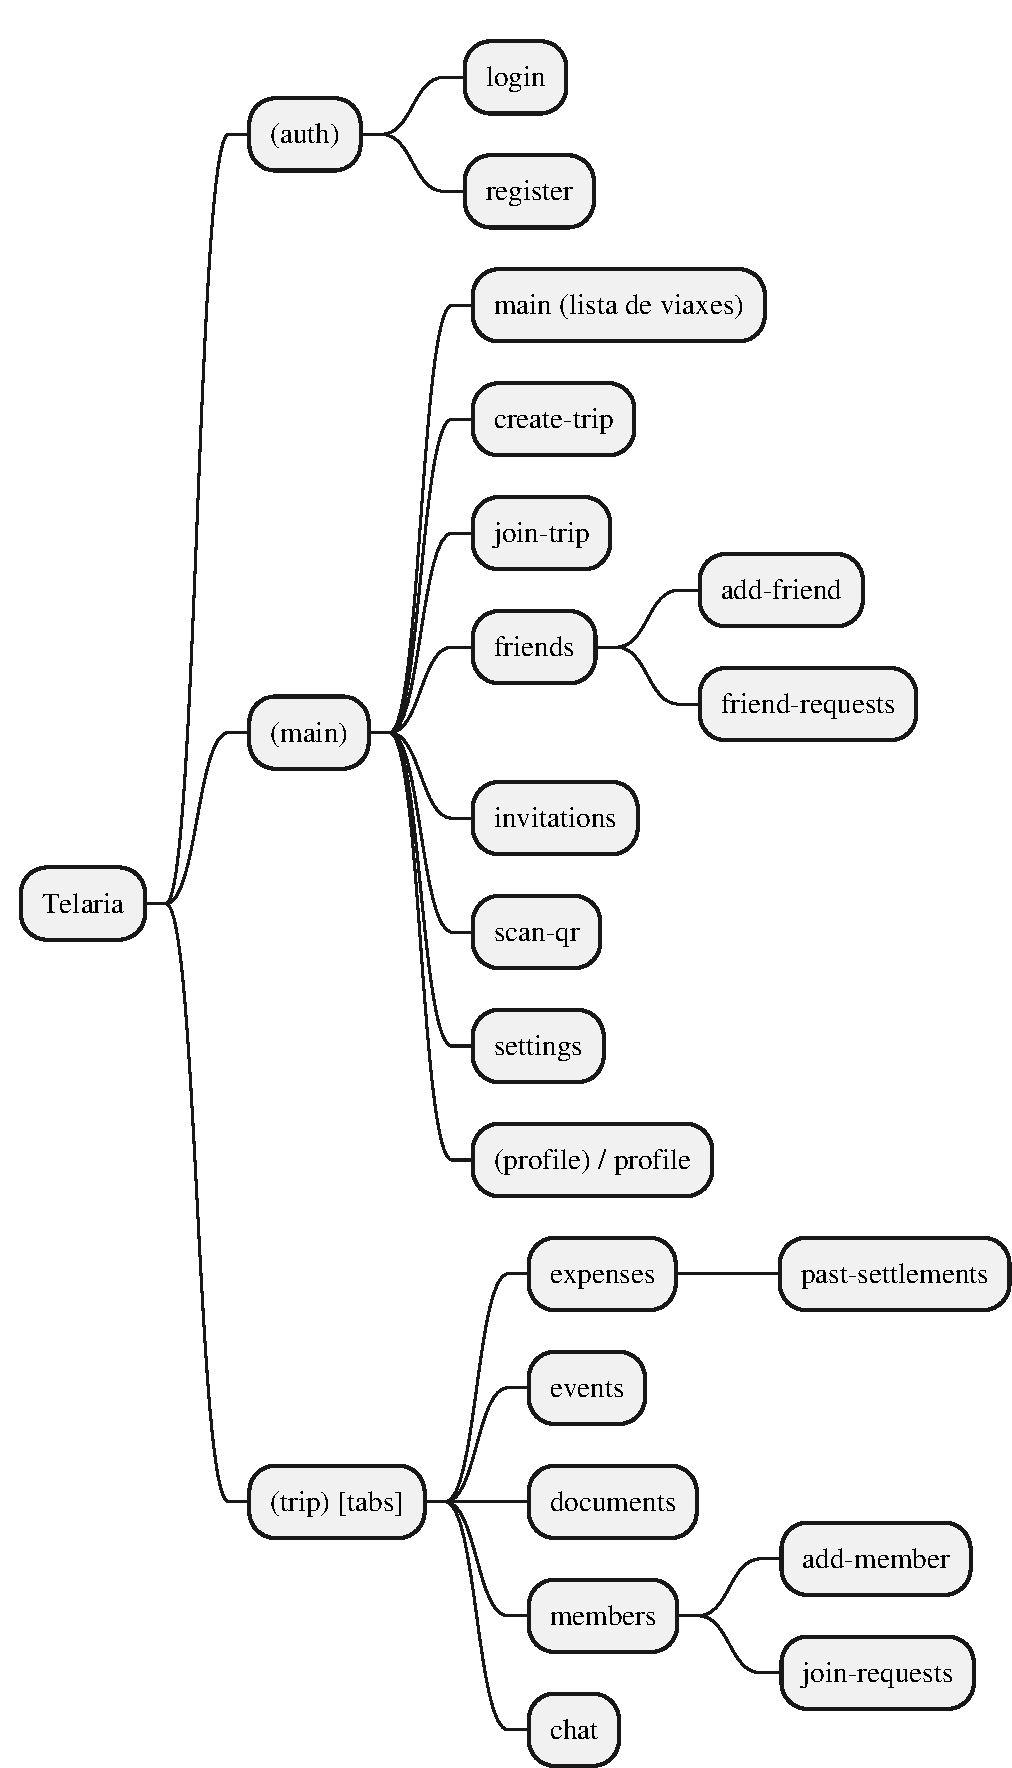
\includegraphics[width=0.55\textwidth]{diagrams/navegacion.pdf}
  \caption{Mapa de navegación da aplicación.}
  \label{fig:navegacion}
\end{figure}

\section{Deseño da interface de usuario}

Alén da súa arquitectura técnica, o frontend conta cunha linguaxe visual propia e coidada.
Nesta sección descríbese o sistema visual, os compoñentes e patróns de interface, as
animacións e a accesibilidade.

\subsection{Linguaxe visual e temas}

A identidade visual de Telaria articúlase arredor dunha paleta monocromática centrada no
violeta. A
aplicación ofrece dous temas (claro e escuro) que o usuario selecciona manualmente e que se
conservan entre sesións (non segue automaticamente o axuste do sistema). A
Figura~\ref{fig:paleta} recolle as cores principais.

\begin{figure}[H]
  \centering
  \renewcommand{\arraystretch}{1.3}
  \begin{tabular}{@{}ll@{}}
    \textbf{Globais}    & \swatch{telPrimary}{\#8b3ce0}\quad\swatch{telWarning}{\#dc2626}\\[6pt]
    \textbf{Tema claro} & \swatch{telLbg}{\#f7f3ff}\quad\swatch{telLui}{\#ede3fd}\quad\swatch{telLtext}{\#3d1e7a}\quad\swatch{telLtint}{\#7c3aed}\quad\swatch{telLborder}{\#d4c2f9}\\[6pt]
    \textbf{Tema escuro}& \swatch{telDbg}{\#07050f}\quad\swatch{telDui}{\#0e0b1f}\quad\swatch{telDtext}{\#e8e0fa}\quad\swatch{telDtint}{\#a855f7}\quad\swatch{telDborder}{\#2b1650}\\
  \end{tabular}
  \caption{Paleta de cores de Telaria: cores globais e específicas de cada tema.}
  \label{fig:paleta}
\end{figure}

A tipografía emprega as fontes do sistema (sen fontes propias) e a xerarquía visual
conséguese mediante o peso e o espazado entre letras, máis que mediante familias
tipográficas distintas. A estética compleméntase con esquinas redondeadas e brillos sutís
(\textit{glow}) de ton violeta arredor dos elementos destacados.

\subsection{Compoñentes e patróns de interface}

A interface constrúese sobre un conxunto de compoñentes reutilizables con tema:
\texttt{ThemedText}, \texttt{ThemedButton} e \texttt{ThemedInput} encapsulan o estilo base;
\texttt{UserAvatar} mostra a imaxe do usuario ou, na súa ausencia, as iniciais, e respecta o
modo de aforro de datos; e \texttt{SegmentedControl} ofrece un selector con animación. O
cromo de navegación componse dunha barra de pestanas inferior que resalta a pestana activa
cun brillo e amosa badges de notificación, e dun menú lateral que se presenta como panel
deslizante inferior (\textit{bottom sheet}). O asistente de IA ábrese nun modal a pantalla
completa accesible desde un botón flotante. Completan o repertorio as tarxetas, os modais e
os diálogos de confirmación. A Figura~\ref{fig:ui-pantalla} mostra unha pantalla representativa.

\begin{figure}[H]\centering
  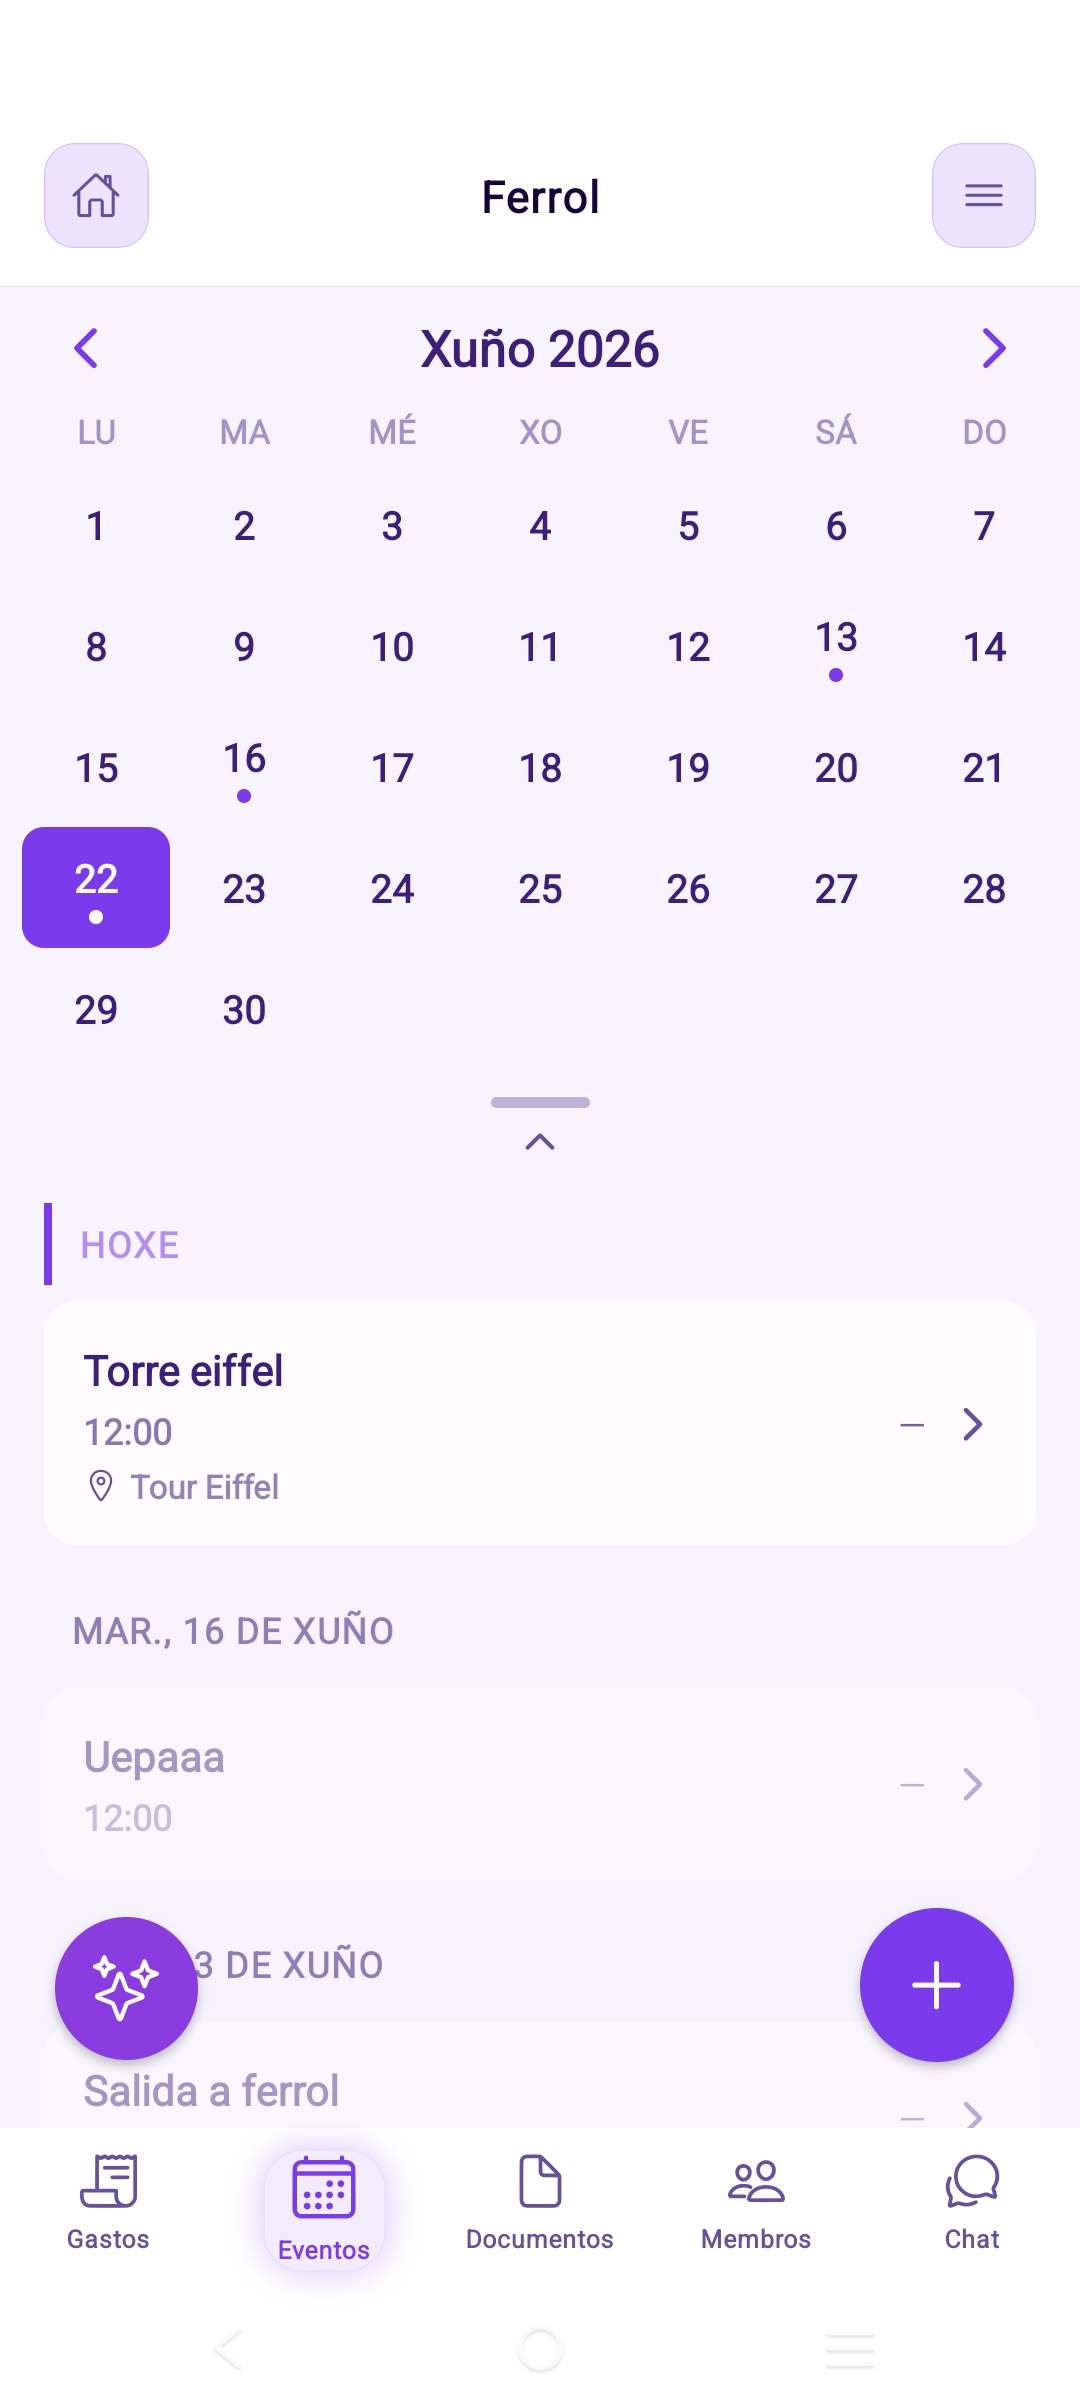
\includegraphics[width=0.45\textwidth]{calendar.jpeg}
  \caption{Pantalla representativa da aplicación (calendario compartido da viaxe).}\label{fig:ui-pantalla}
\end{figure}

\subsection{Animacións e retroalimentación visual}

As animacións baséanse na API \texttt{Animated} de React Native. A retroalimentación de
pulsación aplica unha lixeira redución de escala e de opacidade aos elementos interactivos;
o \texttt{SegmentedControl} desprázase cun efecto de resorte; o escáner de códigos QR mostra
unha liña de varrido e un pulso; o contido reaxústase de forma animada á altura do teclado; e
o fondo das pantallas inclúe unha textura sutil (grella de puntos e manchas de cor ambientais)
que achega profundidade sen distraer.

\subsection{Accesibilidade}

No tocante á accesibilidade, a aplicación adopta varias medidas, aínda que tamén deixa marxe
de mellora que se describe con transparencia.

\textbf{Medidas adoptadas.} A aplicación está internacionalizada en galego, castelán e inglés
(cf.\ RNF-US-02), o que mellora a comprensión para usuarios de distintas linguas. O dobre tema
claro/escuro axuda ás persoas sensibles á luz ou con baixa visión, e o modo de aforro de datos
reduce a carga de imaxes. Ademais, os controis interactivos de toda a aplicación, a barra de
pestanas (que expón a pestana seleccionada mediante \texttt{accessibilityState}), os menús, o
asistente de IA e os botóns de acción das distintas pantallas (engadir, eliminar, navegar,
etc.), incorporan etiquetas (\texttt{accessibilityLabel}) e roles (\texttt{accessibilityRole})
de accesibilidade internacionalizados, de xeito que os lectores de pantalla anuncian cada
control co seu nome; a retroalimentación de pulsación é consistente en toda a interface.
Finalmente, a paleta de cores axustouse para que as combinacións de texto e fondo cumpran o
limiar de contraste \mbox{WCAG~AA}. Ademais, respéctase a preferencia de movemento reducido do
sistema (as animacións desactívanse ou acúrtanse cando o usuario a activa) e as compoñentes de
texto compartidas limitan o factor máximo de escala da tipografía
(\texttt{maxFontSizeMultiplier}) para que os tamaños grandes non rompan os deseños. Os controis
interactivos amplían ademais a súa área de pulsación (\texttt{hitSlop}) ata o tamaño mínimo
recomendado, e as accións consecuentes (saír da viaxe, eliminar a conta, pechar a sesión, etc.)
inclúen pistas (\texttt{accessibilityHint}) que describen o seu efecto.

\textbf{Limitacións.} O límite de escala da tipografía aplícase ás compoñentes de texto
compartidas e aos controis principais, pero aínda non a todos os textos da interface.

\textbf{Traballo futuro.} Unha mellora adicional incluiría estender o límite de escala da
tipografía a todos os textos da interface (e non só ás compoñentes compartidas). Esta revisión
pode apoiarse nas
comprobacións de accesibilidade da ferramenta react-doctor, xa presente no proxecto. A
Figura~\ref{fig:ui-temas} ilustra os dous temas.

\begin{figure}[H]
  \centering
  \subcaptionbox{Tema claro\label{fig:ui-temas-light}}{%
    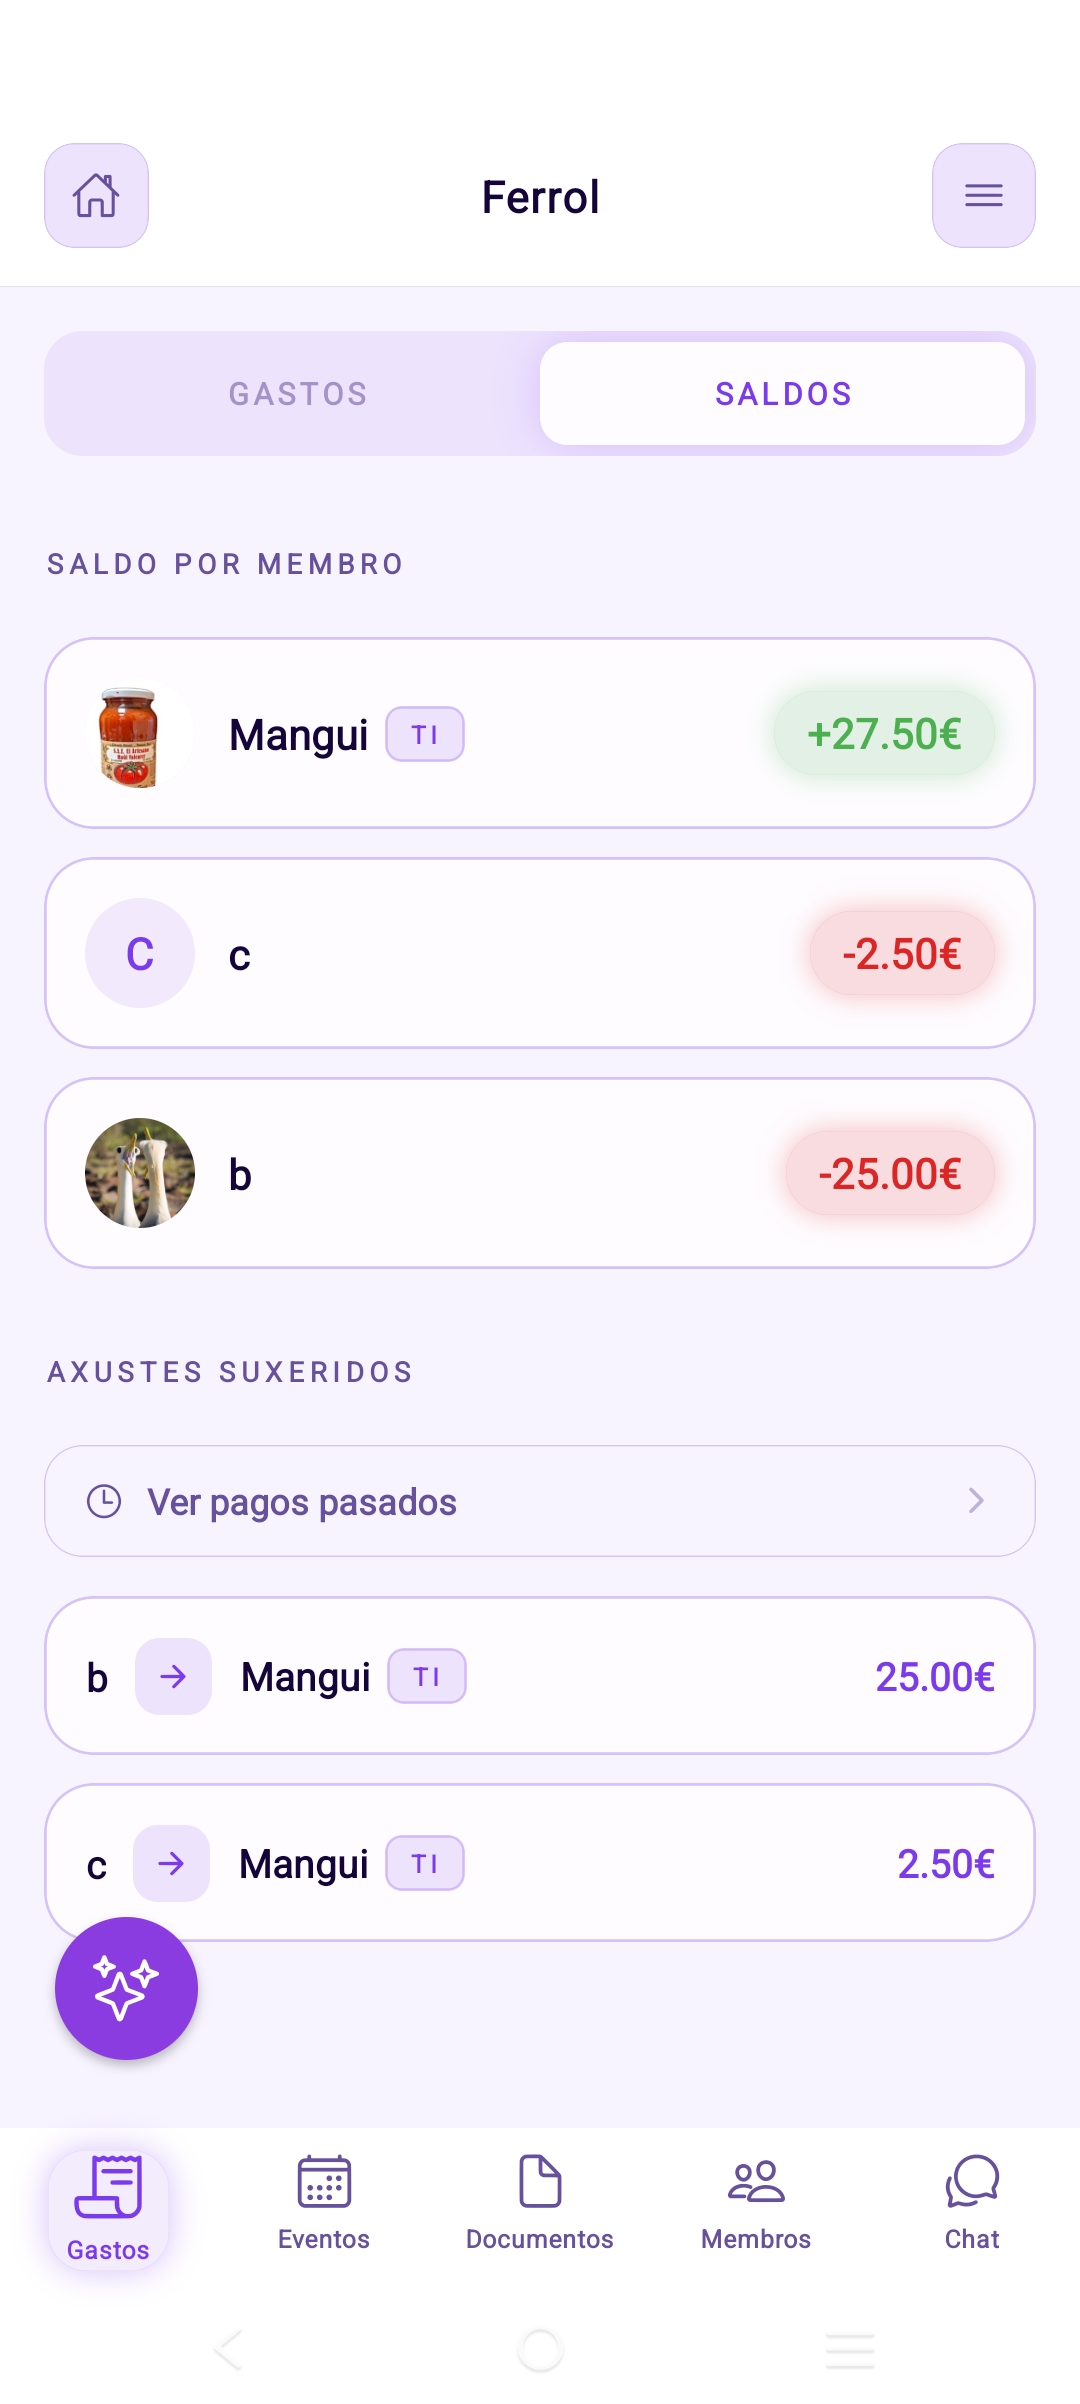
\includegraphics[height=11cm]{balances-light.jpeg}}
  \hspace{0.8cm}
  \subcaptionbox{Tema escuro\label{fig:ui-temas-dark}}{%
    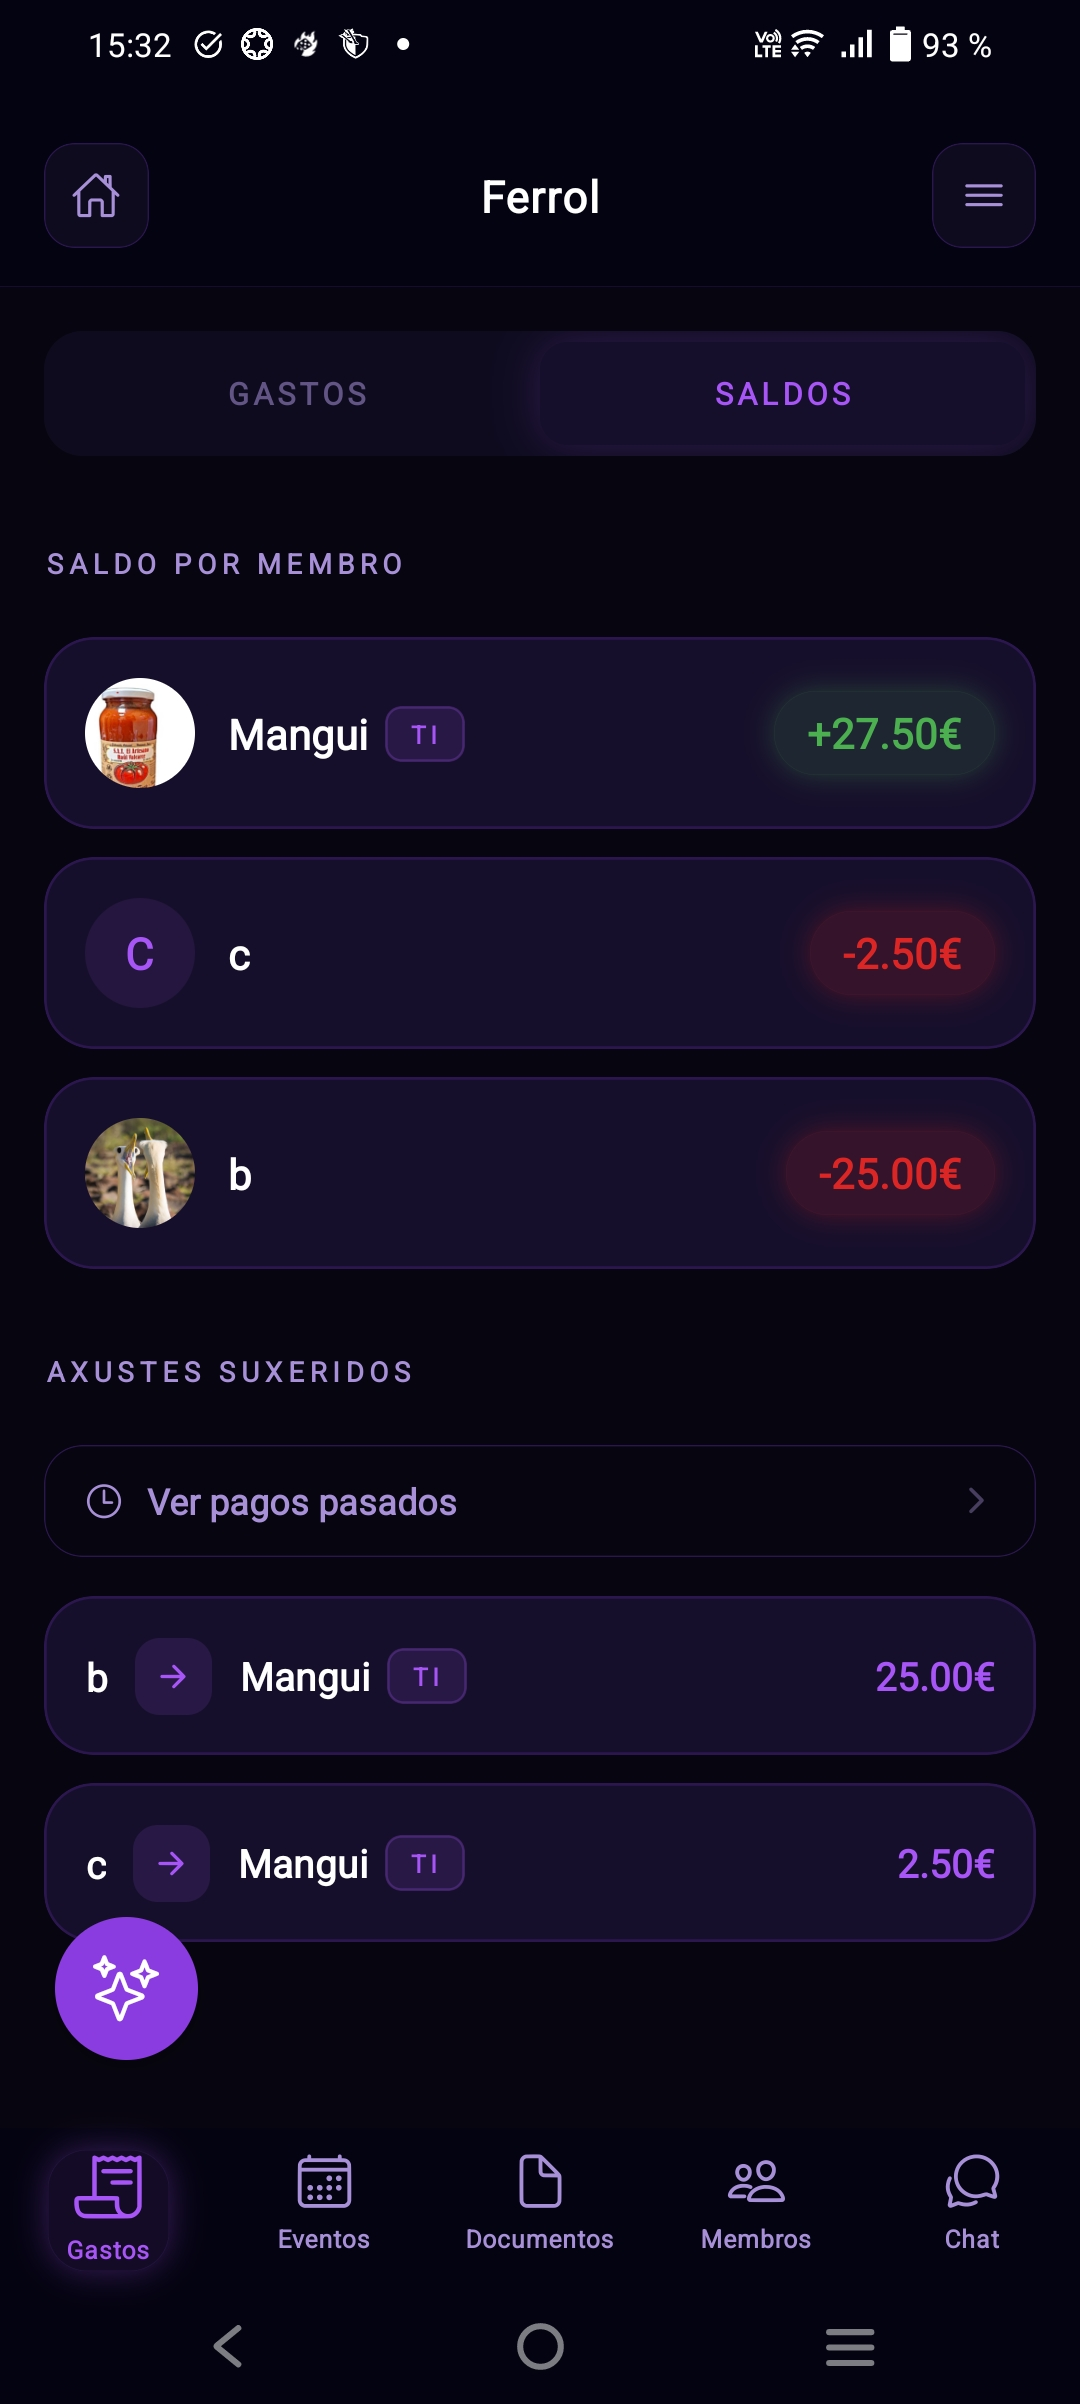
\includegraphics[height=11cm]{balances-dark.jpeg}}
  \caption{Comparación dos temas claro e escuro: pantalla de balances da viaxe.}
  \label{fig:ui-temas}
\end{figure}

\subsection{Análise heurística}

Co obxectivo de identificar posibles problemas de usabilidade desde unha perspectiva
experta, a interface de Telaria avaliouse segundo as \textbf{dez heurísticas de
usabilidade de Nielsen}~\cite{nielsen1994usability}. Esta avaliación complementa as
probas de pensamento en voz alta con usuarios reais descritas no
capítulo~\ref{ch:probas}. A Táboa~\ref{tab:heuristicas} resume como o deseño aborda
cada heurística.

\begin{table}[H]
  \centering
  \begin{tabularx}{\textwidth}{@{}lX@{}}
    \toprule
    \textbf{Heurística} & \textbf{Aplicación en Telaria} \\
    \midrule
    Visibilidade do estado do sistema &
      Indicadores de carga nas chamadas á API, progresión visual na subida de
      documentos, actualizacións en tempo real do chat e do asistente de IA
      (\textit{streaming}) e \textit{badges} de notificación na barra de pestanas. \\
    \addlinespace
    Correspondencia co mundo real &
      Terminoloxía de viaxes familiar (gastos, membros, eventos, calendario),
      categorías de gasto naturais e mapa interactivo para seleccionar localizacións. \\
    \addlinespace
    Control e liberdade do usuario &
      Navegación cara atrás en todos os niveis, posibilidade de abandonar unha viaxe
      e de eliminar a conta, e cancelación de calquera modal sen consecuencias. \\
    \addlinespace
    Consistencia e estándares &
      Compoñentes con tema reutilizables (\texttt{ThemedText}, \texttt{ThemedButton},
      \texttt{ThemedInput}), paleta e tipoloxía uniformes e patróns de navegación
      estándar para plataformas móbiles (barra de pestanas, \textit{bottom sheet}). \\
    \addlinespace
    Prevención de erros &
      Validación de formularios antes do envío, diálogos de confirmación para
      operacións destrutivas (eliminar conta, saír da viaxe) e tipado estrito de
      extremo a extremo a través do contrato OpenAPI. \\
    \addlinespace
    Recoñecemento antes que recordo &
      Barra de pestanas sempre visible, historial de mensaxes e de gastos accesible
      en todo momento e información contextual da viaxe activa presente en cada
      pantalla. \\
    \addlinespace
    Flexibilidade e eficiencia &
      Unión a viaxes por código QR, convites directos a amigos e acceso inmediato
      aos documentos do día seleccionado no calendario. \\
    \addlinespace
    Deseño estético e minimalista &
      Estética limpa, ausencia de información superflua en
      pantalla e textura de fondo sutil que non distrae do contido principal. \\
    \addlinespace
    Axuda para recuperarse de erros &
      Mensaxes de erro claras nas operacións fallidas, formato \textit{Problem
      Details} (RFC~7807)~\cite{rfc7807} nas respostas de erro da API e
      retroalimentación visual ante fallos de rede. \\
    \addlinespace
    Axuda e documentación &
      Asistente de IA integrado que coñece o contexto da viaxe activa (eventos,
      gastos e historial de chat) e pode responder consultas do usuario en
      linguaxe natural. \\
    \bottomrule
  \end{tabularx}
  \caption{Avaliación heurística da interface de Telaria segundo as dez heurísticas de Nielsen.}
  \label{tab:heuristicas}
\end{table}

\section{Fluxos de comunicación entre compoñentes}

\subsection{Autenticación e renovación de tokens}

O inicio de sesión devolve un \textit{access token} JWT de vida curta e un
\textit{refresh token} opaco. Cando o \textit{access token} caduca, o cliente detéctao
ante unha resposta \texttt{401} e renóvao de forma transparente, sen requirir unha nova
autenticación do usuario (Figura~\ref{fig:seq-auth}).

\begin{figure}[H]
  \centering
  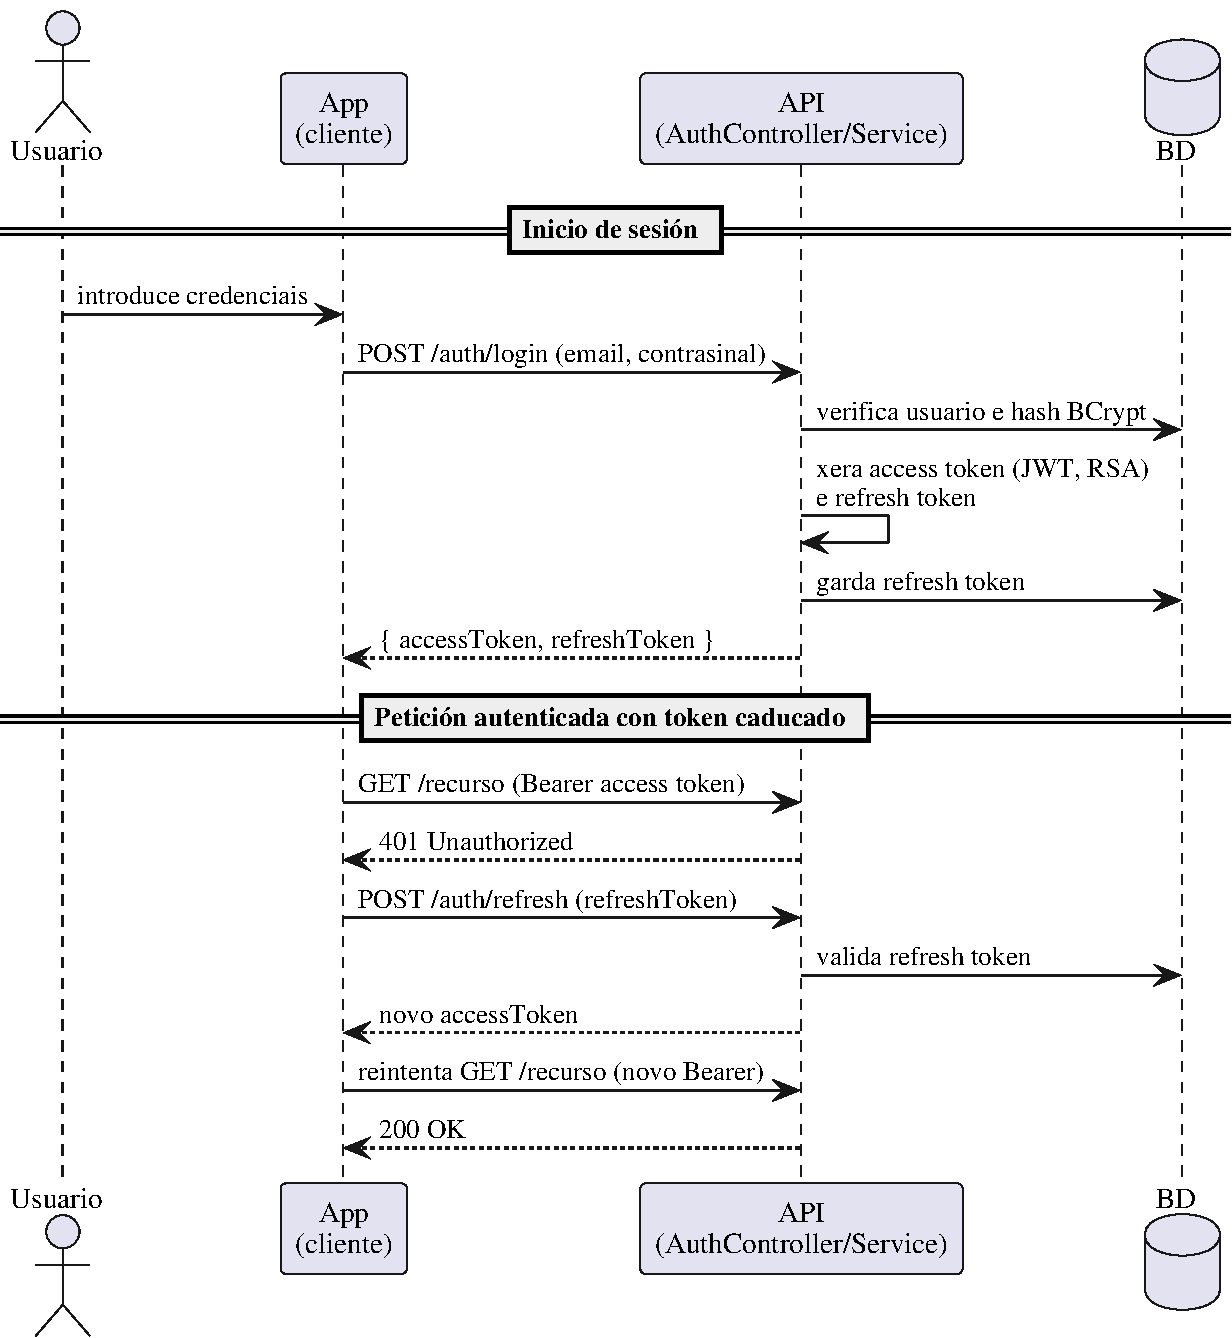
\includegraphics[width=0.7\textwidth]{diagrams/seq-auth.pdf}
  \caption{Secuencia de autenticación e renovación do \textit{access token}.}
  \label{fig:seq-auth}
\end{figure}

\subsection{Chat de grupo en tempo real (SSE)}

Cando un membro abre o chat, o cliente subscríbese a un fluxo SSE. Ao enviar outro membro
unha mensaxe, o servidor persístea e difúndea de inmediato a todos os subscritores
conectados (Figura~\ref{fig:seq-chat}).

\begin{figure}[H]
  \centering
  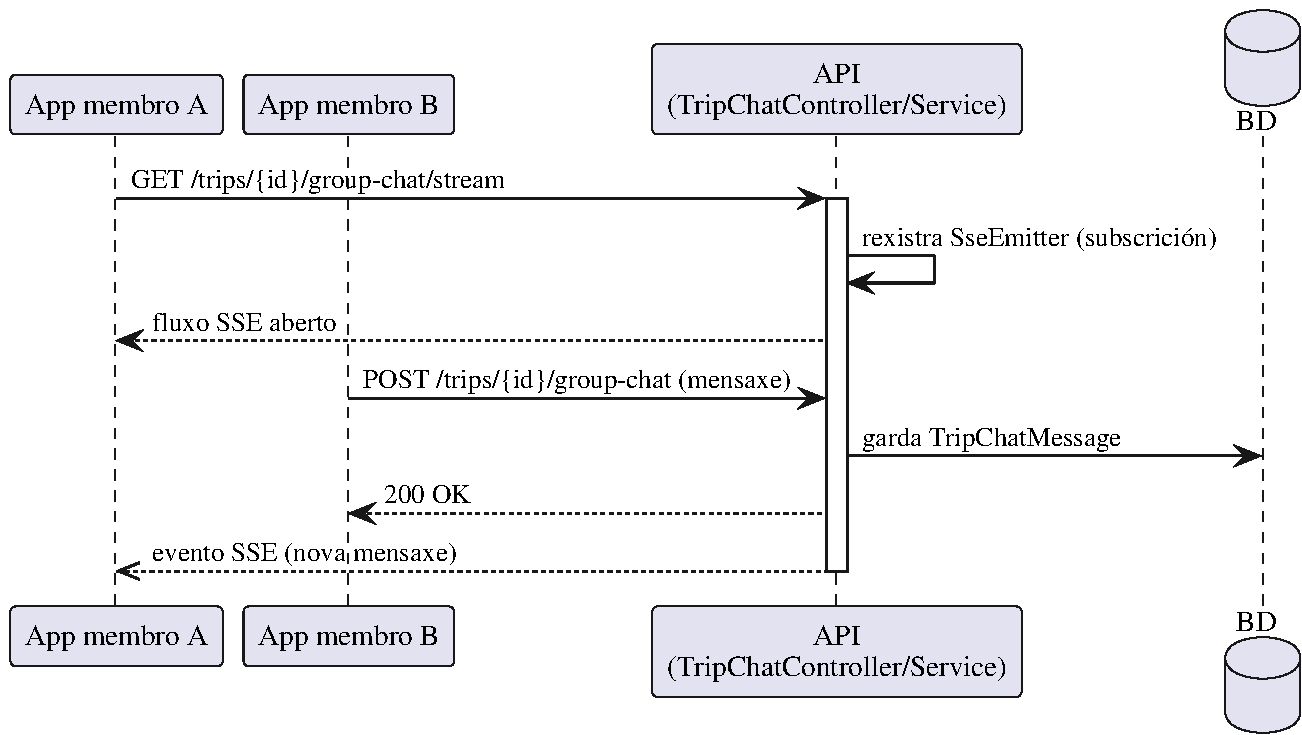
\includegraphics[width=0.8\textwidth]{diagrams/seq-chat-sse.pdf}
  \caption{Secuencia do chat de grupo mediante \textit{Server-Sent Events}.}
  \label{fig:seq-chat}
\end{figure}

\subsection{Subida de documentos con URL prefirmada}

A subida realízase en varios pasos para que o ficheiro non atravese o backend: este crea
o rexistro e devolve unha URL prefirmada, o cliente sobe o ficheiro directamente ao
almacén e, finalmente, confirma a subida; se o ficheiro é unha imaxe, xérase unha
miniatura de forma asíncrona (Figura~\ref{fig:seq-upload}).

\begin{figure}[H]
  \centering
  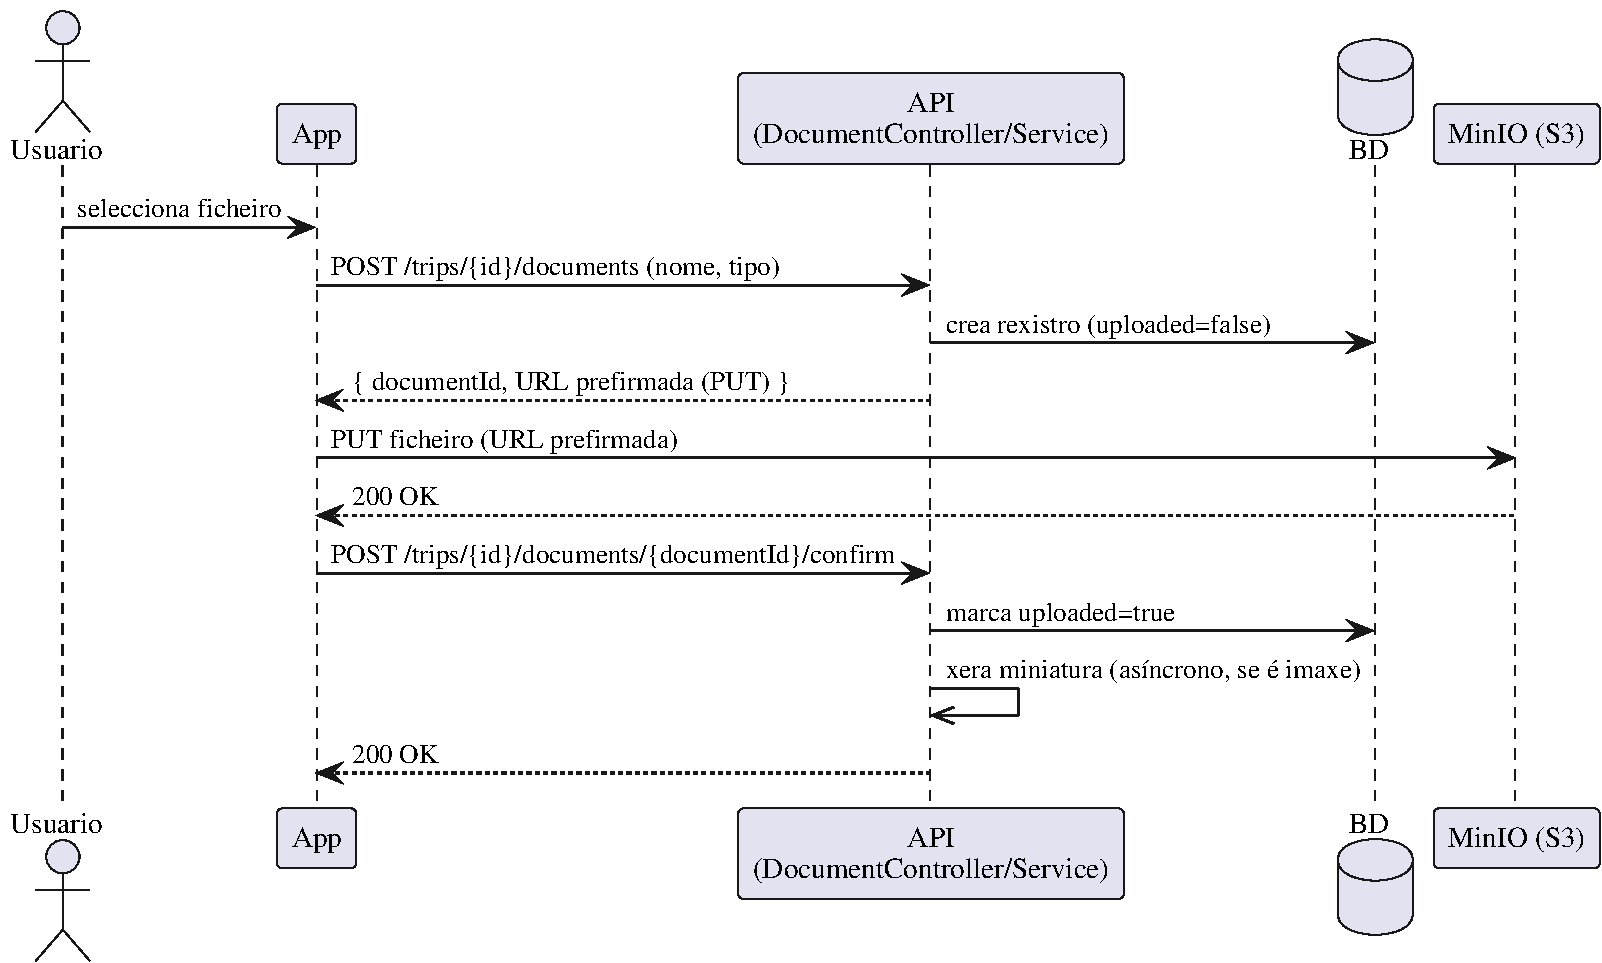
\includegraphics[width=0.9\textwidth]{diagrams/seq-upload.pdf}
  \caption{Secuencia de subida de documentos con URL prefirmada.}
  \label{fig:seq-upload}
\end{figure}

\subsection{Asistente de IA en \textit{streaming}}

Ao recibir unha consulta, o servidor constrúe o contexto da conversa a partir dos
eventos e gastos da viaxe e das últimas mensaxes, e remítello ao modelo local (Ollama). A
resposta devólvese token a token cara ao cliente mediante SSE, ofrecendo unha experiencia
de escritura progresiva (Figura~\ref{fig:seq-ia}).

\begin{figure}[H]
  \centering
  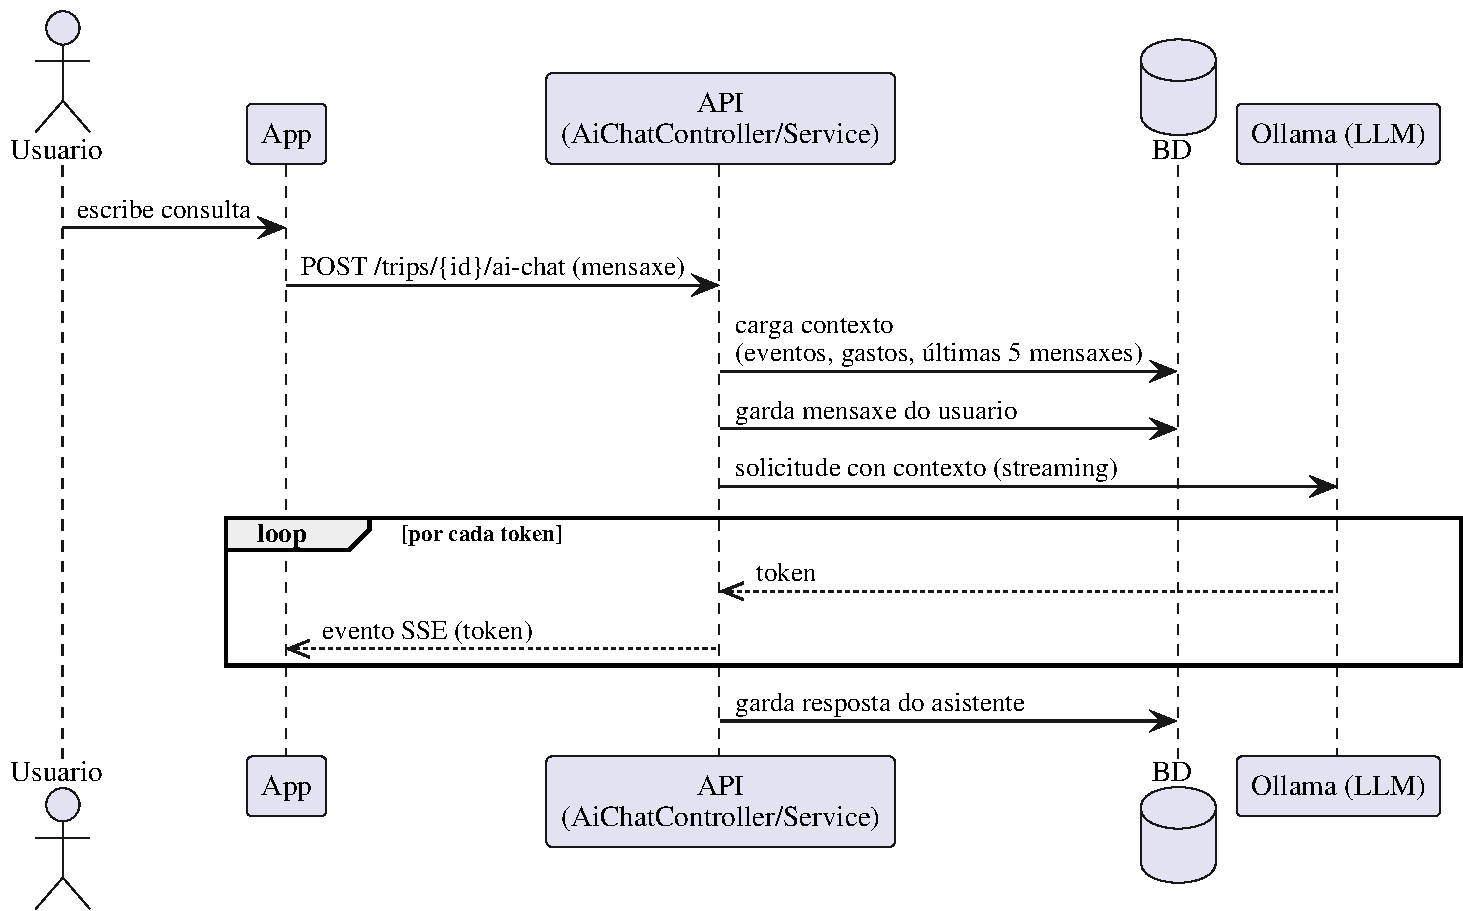
\includegraphics[width=0.85\textwidth]{diagrams/seq-ia.pdf}
  \caption{Secuencia do asistente de IA con resposta en \textit{streaming}.}
  \label{fig:seq-ia}
\end{figure}

\section{Seguridade}

A seguridade do sistema descansa sobre os seguintes piares de deseño:

\begin{itemize}
  \item \textbf{Autenticación con JWT asinado.} No inicio de sesión, o backend asina os
        seus propios \textit{access tokens} (JWT) cunha clave privada RSA almacenada nun
        \textit{keystore}; en cada petición valida a sinatura do token coa clave pública,
        sen necesidade de consultar a base de datos. Esta validación de tokens portadores
        (\textit{bearer}) apóiase no soporte de JWT de Spring Security~\cite{springsecurity}.
        Non se implementa o protocolo OAuth~2.0: non existe un servidor de autorización
        externo nin fluxos de delegación, senón un esquema de autenticación propio baseado
        en tokens autoasinados.
  \item \textbf{Sesións sen estado.} O servidor non mantén sesión; cada petición é
        autosuficiente grazas ao token, o que mellora a escalabilidade.
  \item \textbf{Contrasinais protexidos.} Os contrasinais almacénanse cifrados con
        BCrypt~\cite{bcrypt}.
  \item \textbf{Autorización por pertenza.} O acceso aos recursos dunha viaxe está
        condicionado a que o usuario sexa membro dela.
  \item \textbf{Confirmación en operacións sensibles.} O cambio de correo electrónico e a
        eliminación de conta requiren reintroducir o contrasinal actual.
\end{itemize}

\section{Integración con servizos externos}

\begin{itemize}
  \item \textbf{Ollama.} O asistente de IA delega a inferencia nun modelo de linguaxe
        executado localmente, ao que o backend accede por HTTP en modo \textit{streaming}.
  \item \textbf{Almacén de obxectos (MinIO/S3).} A xestión de ficheiros realízase co AWS
        SDK; o backend nunca recibe nin serve os ficheiros, senón que xera URLs
        prefirmadas de subida e descarga cunha validez limitada.
  \item \textbf{Procesamento de imaxes.} As miniaturas de previsualización e o
        redimensionamento de avatares prodúcense reducindo a imaxe a un tamaño máximo e
        convertíndoa a JPEG, sempre fóra da ruta de petición.
\end{itemize}

\section{Equipamento hardware e software}

O desenvolvemento e a execución do sistema requiren o seguinte equipamento, resumido na
Táboa~\ref{tab:equipamento}. Dado que ningunha destas tecnoloxías constituía un requisito
previo, a súa elección xustifícase nas seccións anteriores e na introdución.

\begin{table}[H]
  \centering
  \begin{tabularx}{\textwidth}{@{}lX@{}}
    \toprule
    \textbf{Ámbito} & \textbf{Tecnoloxías e ferramentas} \\
    \midrule
    Frontend        & React Native, Expo, TypeScript, React Query; ferramentas de Node.js. \\
    Backend         & Java, Spring Boot, Spring Data JPA, Spring Security; construción con Gradle. \\
    Persistencia    & PostgreSQL. \\
    Almacenamento   & MinIO (compatible con S3). \\
    Intelixencia artificial & Ollama (modelo de linguaxe local). \\
    Despregamento   & Contedores OCI xestionados con Podman. \\
    Cliente final   & Dispositivo móbil iOS ou Android con conexión á rede. \\
    \bottomrule
  \end{tabularx}
  \caption{Equipamento software e hardware do sistema.}
  \label{tab:equipamento}
\end{table}

\newpage
\section{Probas}

A verificación da funcionalidade e da corrección global do sistema aborda dúas
dimensións complementarias: as \textbf{probas automatizadas} do backend, que garanten a
corrección técnica da lóxica e da API, e a \textbf{validación funcional} de extremo a
extremo da aplicación, que comproba que o produto se comporta como espera o usuario.

\subsection{Estratexia de probas}

A estratexia segue o modelo da pirámide de probas, con tres niveis:

\begin{itemize}
  \item \textbf{Probas unitarias}: illan a lóxica de negocio de cada servizo, substituíndo
        as dependencias por dobres de proba (\textit{mocks}).
  \item \textbf{Probas de integración (E2E)}: exercitan a API completa contra unha base de
        datos e un almacén de obxectos reais, levantados en contedores efémeros.
  \item \textbf{Validación de sistema}: comprobación manual dos fluxos de usuario completos
        sobre a aplicación en execución.
\end{itemize}

\subsection{Probas automatizadas do backend}

O backend conta cunha batería de \textbf{367 probas automatizadas} repartidas en 26 clases,
que se executan co \textit{framework} JUnit~5. A Táboa~\ref{tab:probas} resume a súa
distribución.

\begin{table}[H]
  \centering
  \begin{tabularx}{\textwidth}{@{}lcX@{}}
    \toprule
    \textbf{Tipo} & \textbf{Clases} & \textbf{Descrición} \\
    \midrule
    Unitarias de servizos   & 10 & Lóxica de negocio illada con Mockito. \\
    Integración (E2E)        & 11 & API completa con base de datos e almacén reais (Testcontainers). \\
    Modelo                   & 3  & Lóxica propia das entidades de dominio. \\
    Tarefas programadas      & 2  & Comportamento dos \textit{schedulers} de limpeza. \\
    \midrule
    \textbf{Total}           & \textbf{26} & \textbf{367 probas} \\
    \bottomrule
  \end{tabularx}
  \caption{Distribución das probas automatizadas do backend.}
  \label{tab:probas}
\end{table}

As probas de integración empregan \textbf{Testcontainers}~\cite{testcontainers}, que levanta
contedores efémeros de PostgreSQL e MinIO para cada execución, de xeito que as probas se
realizan contra servizos reais e non contra simulacións. Unha clase base común
(\texttt{BaseE2ETest}) orquestra o arrinque dos contedores e a aplicación execútase cun
perfil de proba que recrea o esquema da base de datos en cada execución. Deste xeito
verifícanse os fluxos completos da API: autenticación, xestión de viaxes e membros, gastos
e liquidacións, eventos, documentos, chat e asistente de IA.

A cobertura de código mídese con \textbf{JaCoCo}~\cite{jacoco}. A
Táboa~\ref{tab:cobertura} resume os resultados obtidos na execución completa da batería.

\begin{table}[H]
  \centering
  \begin{tabularx}{\textwidth}{@{}Xcc@{}}
    \toprule
    \textbf{Métrica} & \textbf{Cobertura} & \textbf{} \\
    \midrule
    Liñas       & 55,8\,\% & \\
    Instrucións & 48,3\,\% & \\
    Métodos     & 60,7\,\% & \\
    Clases      & 85,5\,\% & \\
    Ramas       & 21,8\,\% & \\
    \bottomrule
  \end{tabularx}
  \caption{Cobertura de código do backend (JaCoCo).}
  \label{tab:cobertura}
\end{table}

A cobertura concéntrase na capa de servizos e nos fluxos principais da API, que é onde
reside a lóxica de negocio. As cifras máis baixas en ramas corresponden, en boa medida, a
ramas defensivas e de manexo de erros pouco frecuentes. Ademais, a construción e a
execución das probas intégranse nun fluxo de integración continua (GitHub Actions), e o
código sométese a análise estática.

\subsection{Validación funcional do sistema}

Para verificar o comportamento de extremo a extremo executáronse manualmente sobre a
aplicación os escenarios de uso descritos na Táboa~\ref{tab:escenarios}, que cobren a
totalidade dos requisitos funcionais. Cada escenario comprende a secuencia completa de
accións do usuario e a comprobación do resultado esperado.

\begin{table}[H]
  \centering
  \begin{tabularx}{\textwidth}{@{}llX@{}}
    \toprule
    \textbf{ID} & \textbf{RF} & \textbf{Escenario verificado} \\
    \midrule
    CP01 & RF01, RF02      & Rexistro, inicio e peche de sesión, e renovación de token. \\
    CP02 & RF03--RF05      & Crear viaxe, convidar e aceptar membros (e por código QR). \\
    CP03 & RF06, RF07      & Rexistrar gastos, consultar balances e liquidar débedas. \\
    CP04 & RF08            & Crear, consultar e eliminar eventos do calendario. \\
    CP05 & RF09            & Subir, previsualizar e eliminar documentos. \\
    CP06 & RF10            & Enviar e recibir mensaxes no chat de grupo en tempo real. \\
    CP07 & RF11            & Conversar co asistente de IA e recuperar o historial. \\
    CP08 & RF12, RF13      & Xestionar amizades e convidar amigos a unha viaxe. \\
    CP09 & RF14, RF15      & Editar o perfil e eliminar a conta con confirmación. \\
    \bottomrule
  \end{tabularx}
  \caption{Escenarios de validación funcional e a súa trazabilidade cos requisitos.}
  \label{tab:escenarios}
\end{table}

\figcaptura{Evidencia da validación funcional (capturas dos escenarios sobre a aplicación)}{fig:evidencia-funcional}

\subsection{Resultados acadados}

A totalidade das \textbf{367 probas automatizadas pasan correctamente}, e os nove
escenarios de validación funcional completáronse co resultado esperado, polo que se
verifica o cumprimento de todos os requisitos funcionais. A cobertura de código do backend
sitúase arredor do 56\,\% de liñas, concentrada na lóxica de negocio.

A principal limitación do plan de probas é a ausencia de probas automatizadas no frontend.
Este risco mitígase por dúas vías: a validación funcional manual descrita anteriormente e a
barreira de tipos que impón o contrato OpenAPI, que detecta en tempo de compilación as
incoherencias entre cliente e servidor. A incorporación de probas automatizadas no frontend
recóllese como liña de mellora nas conclusións.

\chapter{Conclusións e Posibles Ampliacións}

\section{Grao de cumprimento dos obxectivos}

O proxecto acadou os obxectivos formulados na introdución de forma satisfactoria. Telaria centraliza nunha única
aplicación a xestión integral dunha viaxe en grupo, substituíndo o conxunto disperso de
ferramentas que se empregan habitualmente. O Cadro~\ref{tab:obxectivos} resume o grao de
cumprimento de cada obxectivo.

\begin{table}[H]
  \centering
  \caption{Grao de cumprimento dos obxectivos.}
  \label{tab:obxectivos}
  \begin{tabularx}{\textwidth}{@{}p{6.2cm}cX@{}}
    \toprule
    \textbf{Obxectivo} & \textbf{Estado} & \textbf{Observacións} \\
    \midrule
    Gastos compartidos e liquidacións & Cumprido & Cálculo no servidor con minimización de transferencias (RF10, RF11). \\[3pt]
    Calendario de eventos con localización & Cumprido & Eventos con data, duración e localización xeográfica (RF12). \\[3pt]
    Documentos compartidos & Cumprido & Subida directa ao almacén con miniaturas (RF13). \\[3pt]
    Chat de grupo & Cumprido & Mensaxería en tempo real mediante SSE (RF14). \\[3pt]
    Asistente de IA por viaxe & Cumprido & Chatbot con historial persistente sobre Ollama (RF15). \\[3pt]
    Rede de amizades (complementaria) & Cumprido & Solicitudes, lista de amigos e convite áxil (RF16, RF17). \\[3pt]
    Xestión de conta & Cumprido & Perfil, contrasinal, avatar e eliminación con confirmación (RF03, RF04). \\[3pt]
    Arquitectura API-first & Cumprido & Contrato OpenAPI con xeración de código en ambos os extremos. \\[3pt]
    Multiplataforma iOS/Android & Cumprido & Única base de código con React Native e Expo. \\
    \bottomrule
  \end{tabularx}
\end{table}

\section{Valoración técnica}

A adopción dunha arquitectura \textit{API-first} demostrou ser un acerto: ter o contrato
OpenAPI como fonte de verdade permitiu xerar automaticamente os tipos do cliente e as
interfaces do servidor, mantendo ambos os extremos sincronizados e detectando
incoherencias en tempo de compilación. O uso de \textit{Server-Sent Events} para o chat e
o asistente de IA, e o das URLs prefirmadas para os ficheiros, permitiron implementar
funcionalidades esixentes sen sobrecargar o servidor. A execución local do modelo de
linguaxe con Ollama evitou a dependencia de servizos externos de pago. Finalmente, a
batería de probas automatizadas do backend proporcionou unha rede de seguridade que
facilitou a evolución continua do código.

Entre as dificultades atopadas destacan a integración de Testcontainers cun entorno de
contedores sen daemon (Podman), a coordinación dos fluxos asíncronos de \textit{streaming}
e a xestión coherente da subida de ficheiros en varios pasos.

\section{Posibles ampliacións}

O sistema deixa aberto un conxunto de liñas de mellora:

\begin{itemize}
  \item \textbf{Notificacións push} para invitacións, mensaxes novas e recordatorios de eventos.
  \item \textbf{Preparación para produción}: externalizar os segredos de configuración
        (actualmente en ficheiros de configuración), habilitar HTTPS/TLS e facer
        configurable a dirección do servidor no cliente. Empregar servizos de hosting para o backend que permitan escalar a demanda,
        mellores modelos para o asistente de IA, monitorización de métricas e alertas, etc. O frontend
            tamén debería ser empaquetado e publicado en \textit{App Store} e \textit{Google Play}.
  \item \textbf{Engadir as probas do frontend ao pipeline de desenvolvemento}: Debido a limitacións 
       de tempo e á tardía implementación das probas do frontend polo seu carácter máis propenso a cambios e
       rediseños, non se puideron integrar estas no pipeline de desenvolvemento.
   A súa integración permitiría detectar erros de interface e de interacción de usuario antes de que cheguen á produción.
  \item \textbf{Modo sen conexión} con sincronización posterior, para mellorar a
        experiencia en destinos con conectividade limitada.
  \item \textbf{Accesibilidade}: Mellorar a accesibilidade tendo en conta diversos perfís de
        usuario con distintas dificultades (engadir un modo para daltónicos, etc.).
  \item \textbf{Integración de provedores de identidade}: Permitir o inicio de sesión mediante provedores externos como Google ou Meta.
  \item \textbf{Soporte web}: Aínda que a aplicación está pensada para dispositivos móbiles, un cliente web permitiría acceder á información dende calquera navegador.
\end{itemize}


% ====================== Apéndices (manuais, fóra do límite) ===================
\appendix
\chapter{Manual técnico}

Este manual recolle a información necesaria para instalar, executar, probar e modificar
Telaria. Diríxese a persoas que vaian continuar o desenvolvemento do sistema.

\section{Requisitos do entorno}

\begin{itemize}
  \item \textbf{JDK 25} (para o backend; a construción realízase co \textit{wrapper} de Gradle).
  \item \textbf{Node.js} con \texttt{npm} (para o frontend e a xeración de tipos).
  \item \textbf{Podman} con soporte de \texttt{podman compose} (para os servizos de apoio).
  \item \textbf{Git}.
\end{itemize}

\section{Estrutura do repositorio}

\begin{itemize}
  \item \texttt{backend/} — API REST en Spring Boot (Gradle).
  \item \texttt{frontend/} — aplicación móbil en React Native + Expo.
  \item \texttt{memoria/} — esta documentación (LaTeX).
\end{itemize}

\section{Servizos de apoio (Podman)}

Os servizos auxiliares (PostgreSQL, MinIO e Ollama) defínense en
\texttt{backend/compose.yaml}. O xeito máis sinxelo de poñelos en marcha, descargar o
modelo de linguaxe e arrincar o backend é o \textit{script} de inicio:

\begin{lstlisting}[language=bash]
cd backend
./start.sh
\end{lstlisting}

\noindent Alternativamente, pódense levantar só os contedores:

\begin{lstlisting}[language=bash]
cd backend
podman compose up -d        # engadir --profile gpu se hai GPU dispoñible
\end{lstlisting}

\noindent Portos por defecto: PostgreSQL \texttt{5432}, MinIO \texttt{9000}/\texttt{9001}
(API/consola), Ollama \texttt{11434}.

\section{Execución do backend}

\begin{lstlisting}[language=bash]
cd backend
./gradlew bootRun
\end{lstlisting}

\noindent O servidor escoita no porto \texttt{8082}. A configuración (base de datos,
\textit{keystore} de sinatura JWT, MinIO e tarefas programadas) atópase en
\texttt{src/main/resources/application.yaml}. A documentación interactiva da API queda
dispoñible en \texttt{/swagger-ui.html}.

\section{Execución do frontend}

\begin{lstlisting}[language=bash]
cd frontend
npm install
npm start            # inicia o servidor de desenvolvemento de Expo
\end{lstlisting}

\noindent A dirección do backend configúrase na constante \texttt{BASE\_URL} de
\texttt{frontend/constants/constants.tsx}, que debe apuntar ao enderezo accesible do
servidor desde o dispositivo. A aplicación pode abrirse en Expo Go ou nun emulador
(\texttt{npm run android} / \texttt{npm run ios}).

\section{Contrato OpenAPI e xeración de código}

A API especifícase en \texttt{backend/src/main/resources/openapi/}, cun documento
principal (\texttt{api.yaml}) que referencia ficheiros de rutas e esquemas. A partir del
xérase código:

\begin{lstlisting}[language=bash]
# Backend: interfaces de controladores e DTO
cd backend && ./gradlew openApiGenerate

# Frontend: tipos TypeScript
cd frontend && npm run generate:types
\end{lstlisting}

\noindent Ao editar ficheiros referenciados con \texttt{\$ref} (rutas ou esquemas), pode
ser preciso forzar a rexeneración, xa que a tarefa de Gradle só observa cambios en
\texttt{api.yaml}.

\section{Execución das probas}

As probas de integración (E2E) empregan Testcontainers, que require un \textit{socket}
compatible con Docker. Con Podman \textit{rootless}, débese indicar a súa ruta:

\begin{lstlisting}[language=bash]
cd backend
export DOCKER_HOST=unix:///run/user/$(id -u)/podman/podman.sock
export TESTCONTAINERS_RYUK_DISABLED=true
./gradlew test
\end{lstlisting}

\noindent Ao rematar, o informe de cobertura JaCoCo xérase en
\texttt{backend/build/reports/jacoco/test/html/index.html}. A análise estática SpotBugs
está dispoñible mediante a tarefa correspondente de Gradle.

\section{Configuración e segredos}

A configuración do backend (credenciais da base de datos, contrasinal do \textit{keystore}
JWT, claves de acceso a MinIO e parámetros das tarefas programadas) reside en
\texttt{application.yaml}. Para un despregamento en produción recoméndase externalizar
estes valores mediante variables de entorno e non incluílos no control de versións.

\section{Integración continua}

O repositorio inclúe fluxos de traballo de GitHub Actions que executan a construción e as
probas do backend, así como unha análise de seguridade do código (CodeQL).

\newpage
\section{Manual de usuario}

Este manual é autocontido e está dirixido ás persoas que utilicen Telaria. Describe a
instalación e o uso de todas as funcionalidades. As capturas de pantalla insírense nos
espazos reservados ao efecto.

\subsection{Instalación e acceso}

Telaria é unha aplicación móbil para iOS e Android. Durante o desenvolvemento pode
executarse a través de Expo Go ou instalando unha compilación da aplicación. Ao abrila por
primeira vez, o usuario debe rexistrarse ou iniciar sesión.

\subsection{Rexistro e inicio de sesión}

Na pantalla inicial pódese crear unha conta nova indicando nome de usuario, correo
electrónico e contrasinal (con confirmación), ou iniciar sesión cunha conta existente. A
sesión mantense aberta entre usos.

\figcaptura{Pantallas de rexistro e inicio de sesión}{fig:b-login}

\subsection{Pantalla principal: as miñas viaxes}

Tras iniciar sesión, móstrase a lista de viaxes do usuario. Desde aquí pódese acceder a
unha viaxe, crear unha nova ou unirse a unha existente, así como abrir o menú lateral para
acceder a amigos, invitacións, perfil e axustes.

\figcaptura{Lista de viaxes e menú principal}{fig:b-main}

\subsection{Crear e unirse a viaxes}

Para crear unha viaxe abonda con indicar o seu nome; opcionalmente pódense convidar amigos
no momento da creación. Para unirse a unha viaxe existente pódese empregar unha invitación
recibida, enviar unha solicitude de unión ou escanear un código QR.

\figcaptura{Creación de viaxe e unión mediante código QR}{fig:b-crear}

\subsection{Xestión de membros}

Dentro dunha viaxe, calquera membro pode convidar outros usuarios e xestionar as
solicitudes de unión pendentes. Non existen roles: todos os membros teñen as mesmas
capacidades.

\figcaptura{Membros da viaxe e solicitudes pendentes}{fig:b-membros}

\subsection{Gastos e liquidacións}

No apartado de gastos rexístranse os pagamentos indicando importe, concepto, categoría,
quen pagou e entre quen se reparte. A aplicación calcula automaticamente os balances (quen
debe a quen) e propón as liquidacións que minimizan o número de transferencias. As débedas
saldadas rexístranse no histórico de liquidacións.

\figcaptura{Lista de gastos, balances e liquidacións}{fig:b-gastos}

\subsection{Eventos e calendario}

O calendario da viaxe permite crear eventos con nome, data e hora de inicio, duración e
unha localización opcional. Os eventos amósanse organizados por data.

\figcaptura{Calendario e creación de eventos}{fig:b-eventos}

\subsection{Documentos compartidos}

Os membros poden subir documentos relevantes para a viaxe (reservas, billetes, etc.) e
consultalos ou eliminalos. Os documentos de imaxe amosan unha miniatura de previsualización.

\figcaptura{Listaxe de documentos compartidos}{fig:b-documentos}

\subsection{Chat de grupo}

Cada viaxe dispón dun chat común no que os membros intercambian mensaxes en tempo real.

\figcaptura{Chat de grupo da viaxe}{fig:b-chat}

\subsection{Asistente de intelixencia artificial}

Cada viaxe inclúe un asistente conversacional que responde preguntas tendo en conta o
contexto da viaxe (eventos e gastos). A conversa garda un historial persistente.

\figcaptura{Asistente de IA da viaxe}{fig:b-ia}

\subsection{Amizades}

A sección de amigos permite enviar e xestionar solicitudes de amizade (por identificador
ou código QR), consultar a lista de amigos e eliminar amizades. Os amigos poden convidarse
ás viaxes de forma máis áxil.

\figcaptura{Lista de amigos e solicitudes de amizade}{fig:b-amigos}

\subsection{Perfil e axustes}

No perfil pódese consultar e actualizar o nome de usuario e o correo electrónico (o cambio
de correo require o contrasinal), cambiar o contrasinal e establecer un avatar. Nos axustes
configúrase o idioma (galego, castelán ou inglés), o tema (claro ou escuro) e o aforro de
datos.

\figcaptura{Perfil de usuario e pantalla de axustes}{fig:b-perfil}

\subsection{Eliminación da conta}

Desde os axustes, o usuario pode eliminar a súa conta. A operación require a confirmación
do contrasinal e elimina os datos persoais asociados.

\figcaptura{Confirmación de eliminación de conta}{fig:b-eliminar}

\subsection{Mensaxes de erro comúns}

\begin{itemize}
  \item \textbf{Credenciais incorrectas}: o correo ou o contrasinal non son válidos no
        inicio de sesión.
  \item \textbf{Correo xa rexistrado}: existe xa unha conta con ese correo ao rexistrarse.
  \item \textbf{Acción xa realizada}: por exemplo, o usuario xa é membro da viaxe ou xa foi
        convidado.
  \item \textbf{Sen conexión}: a aplicación require conexión á rede; comprobe a
        conectividade e que o servidor estea accesible.
\end{itemize}

\chapter{Licenza}

% TODO: texto da licenza (GNU GPL, Creative Commons, etc.)


% ====================== Bibliografía ==========================================
\cleardoublepage
\newpage
\renewcommand{\refname}{Bibliografía}
\addcontentsline{toc}{section}{Bibliografía}
\begin{thebibliography}{99}

\bibitem{reactnative} Meta Platforms, Inc. \emph{React Native — A framework for building native apps using React}. \url{https://reactnative.dev}

\bibitem{expo} Expo. \emph{Expo Documentation}. \url{https://docs.expo.dev}

\bibitem{reactquery} TanStack. \emph{TanStack Query (React Query)}. \url{https://tanstack.com/query}

\bibitem{springboot} Broadcom (VMware Tanzu). \emph{Spring Boot Reference Documentation}. \url{https://spring.io/projects/spring-boot}

\bibitem{springsecurity} Broadcom (VMware Tanzu). \emph{Spring Security Reference Documentation}. \url{https://spring.io/projects/spring-security}

\bibitem{openapi} OpenAPI Initiative. \emph{OpenAPI Specification}. \url{https://spec.openapis.org}

\bibitem{postgresql} The PostgreSQL Global Development Group. \emph{PostgreSQL Documentation}. \url{https://www.postgresql.org/docs/}

\bibitem{rfc7519} M. Jones, J. Bradley e N. Sakimura. \emph{JSON Web Token (JWT)}. RFC~7519, IETF, 2015. \url{https://www.rfc-editor.org/rfc/rfc7519}

\bibitem{rfc7807} M. Nottingham e E. Wilde. \emph{Problem Details for HTTP APIs}. RFC~7807, IETF, 2016. \url{https://www.rfc-editor.org/rfc/rfc7807}

\bibitem{ollama} Ollama. \emph{Ollama — Get up and running with large language models locally}. \url{https://ollama.com}

\bibitem{minio} MinIO, Inc. \emph{MinIO Object Storage Documentation}. \url{https://min.io}

\bibitem{bcrypt} N. Provos e D. Mazières. \emph{A Future-Adaptable Password Scheme}. Proceedings of the USENIX Annual Technical Conference, 1999.

\bibitem{podman} Red Hat, Inc. \emph{Podman — A tool for managing OCI containers and pods}. \url{https://podman.io}

\bibitem{testcontainers} AtomicJar / Docker, Inc. \emph{Testcontainers for Java}. \url{https://java.testcontainers.org}

\bibitem{jacoco} \emph{JaCoCo Java Code Coverage Library}. \url{https://www.jacoco.org/jacoco/}

\end{thebibliography}


\end{document}
